% Chapter Template

\chapter{Results and discussions} % Main chapter title

\label{Chapter4} % Change X to a consecutive number; for referencing this chapter elsewhere, use \ref{ChapterX}

%----------------------------------------------------------------------------------------
%	SECTION 1
%----------------------------------------------------------------------------------------

\red{
    To be defined: \\
    Chirp pass \\
    Gravitational and Baryonic masses
}

In this chapter we review the findings of \citet{Nedora:2019jhl} and \citet{Nedora:2020pak}
and investigate the long-term \pmerg{} evolution of the binary neutron star. 

Such studies are of high astrophysical importance as the ejecta of matter that occur 
on various timescales \pmerg{} undergoes \rproc{} and produces observable EM emission. 
The discussion of the \rproc{} and EM transits themselves, we resort for the chapter \red{chap:coutnerparts}.


\section{Simulations}



%% --------------------------------
%% TAB SIM SUMMARY
%\begin{table*}
\begin{sidewaystable}
\begin{center}
\captionsetup{width=1.0\linewidth}
    \caption{
      Summary table of all the simulations and dynamical ejecta properties. The columns contain
      the following information, starting from the left. Equation of
      state, mass-ratio, available resolutions,
      inclusion of subgrid turbulence, time of the
      simulation end, time of the BH formation for LR, SR, HR
      resolutions separately, time of last output, time the disk mass
      is extracted, disk mass, mass of the
      dynamical ejecta, mass-averaged electron fracton, terminal
      velocity and RMS angle (from the binary plane) for dynamical ejecta. For all
      data except $t_{BH}$, $t_{\text{end}}$ and $t_{\text{disk}}$, the value that is given is a mean value across resolutions, with an error estimated as one
      standard diviaion from the mean. In case where only one
      resolution is present, the error is assumed to be $20\%$ of the
      value. Adopted from \citet{Nedora:2020pak}.
    }
      %% \newtxt{For discussions on errors and convergence see \citep{Radice:2018pdn,Bernuzzi:2020txg}.
      %% The model data are available online at \citep{vsevolod_nedora_2020_4159619}.
%%       }
\scalebox{0.70}{
\begin{tabular}{c c c c c c c c c c c c c}
    \hline\hline
    EOS & $q$ & $\tilde{\Lambda}$ & Resolution & GRLES & $t_{\text{end}}$ & $t_{\text{BH}}$ & $t_{\text{disk}}$ & $M_{\text{disk}} ^{\text{last}}$ & $\md$ & $\langle \yd \rangle$ & $\langle \vd  \rangle$ & $\langle \theta_{\text{ej}} ^{\text{d}} \rangle$ \\
    &   &   &  &  & [ms] & [ms] & [ms] &   & $[10^{-2} M_{\odot}]$ &   & $[c]$ &   \\ 
    \hline
    \hline
    BLh & 1.00 & 541 & \texttt{LR SR HR} & \cmark & $43.3$ $91.8$ $23.1$ & $>43.3$ $>91.8$ $>23.1$ & 23.1 & $0.166^{+0.052} _{-0.052} $ & $0.14^{+0.02} _{-0.02} $ & $0.27^{+0.01} _{-0.01} $ & $0.17^{+0.01} _{-0.01} $ & $39.65^{+0.35} _{-0.35} $ \\
    BLh & 1.00 & 541 & \texttt{LR SR} & \xmark & $15.9$ $103.2$ $ $ & $>15.9$ $>103.2$ $ $ & 15.6 & $0.261^{+0.008} _{-0.008} $ & $0.12^{+0.01} _{-0.01} $ & $0.27^{+0.01} _{-0.01} $ & $0.16^{+0.01} _{-0.01} $ & $38.80^{+0.44} _{-0.44} $ \\
%%  BLh & 1.00 & 541 & \texttt{LR SR} & \xmark & $36.9$ $15.5$ $ $ & $>36.9$ $>15.5$ $ $ & 36.6 & $0.182^{+0.091} _{-0.091} $ & $0.21^{+0.04} _{-0.04} $ & $0.26^{+0.01} _{-0.01} $ & $0.18^{+0.01} _{-0.01} $ & $36.29^{+0.24} _{-0.24} $ \\
    \hline
    BLh & 1.18 & 539 & \texttt{LR} & \cmark & $69.4$ $ $ $ $ & $>69.4$ $ $ $ $ & 69.0 & $0.202^{+0.101} _{-0.101} $ & $0.30^{+0.06} _{-0.06} $ & $0.18^{+0.04} _{-0.04} $ & $0.19^{+0.04} _{-0.04} $ & $33.65^{+6.73} _{-6.73} $ \\
    BLh & 1.18 & 539 & \texttt{LR} & \xmark & $16.4$ $ $ $ $ & $>16.4$ $ $ $ $ & 15.9 & $0.229^{+0.115} _{-0.115} $ & $0.25^{+0.05} _{-0.05} $ & $0.16^{+0.03} _{-0.03} $ & $0.20^{+0.04} _{-0.04} $ & $30.86^{+6.17} _{-6.17} $ \\
    \hline
    BLh & 1.34 & 539 & \texttt{LR SR} & \cmark & $63.4$ $9.8$ $ $ & $>63.4$ $>9.8$ $ $ & 9.8 & $0.192^{+0.004} _{-0.004} $ & $0.25^{+0.05} _{-0.05} $ & $0.14^{+0.04} _{-0.04} $ & $0.17^{+0.00} _{-0.00} $ & $28.79^{+5.00} _{-5.00} $ \\
    BLh & 1.34 & 539 & \texttt{LR} & \xmark & $18.0$ $ $ $ $ & $>18.0$ $ $ $ $ & 18.0 & $0.211^{+0.106} _{-0.106} $ & $0.19^{+0.04} _{-0.04} $ & $0.17^{+0.03} _{-0.03} $ & $0.17^{+0.03} _{-0.03} $ & $33.39^{+6.68} _{-6.68} $ \\
    \hline
    BLh & 1.43 & 540 & \texttt{LR SR} & \cmark & $35.1$ $59.6$ $ $ & $>35.1$ $>59.6$ $ $ & 33.8 & $0.265^{+0.001} _{-0.001} $ & $0.27^{+0.08} _{-0.08} $ & $0.19^{+0.03} _{-0.03} $ & $0.16^{+0.00} _{-0.00} $ & $34.49^{+3.59} _{-3.59} $ \\
    \hline
    BLh & 1.54 & 543 & \texttt{LR} & \cmark & $45.8$ $ $ $ $ & $>45.8$ $ $ $ $ & 53.8 & $0.324^{+0.162} _{-0.162} $ & $0.20^{+0.04} _{-0.04} $ & $0.17^{+0.03} _{-0.03} $ & $0.13^{+0.03} _{-0.03} $ & $31.21^{+6.24} _{-6.24} $ \\
    BLh & 1.54 & 543 & \texttt{LR} & \xmark & $17.4$ $ $ $ $ & $>17.4$ $ $ $ $ & 30.1 & $0.287^{+0.144} _{-0.144} $ & $0.22^{+0.04} _{-0.04} $ & $0.21^{+0.04} _{-0.04} $ & $0.16^{+0.03} _{-0.03} $ & $35.05^{+7.01} _{-7.01} $ \\
    \hline
    BLh & 1.66 & 538 & \texttt{LR SR} & \cmark & $64.6$ $20.1$ $ $ & $>64.6$ $1.8$ $ $ & 19.2 & $0.289^{+0.005} _{-0.005} $ & $0.42^{+0.05} _{-0.05} $ & $0.11^{+0.01} _{-0.01} $ & $0.12^{+0.01} _{-0.01} $ & $24.08^{+0.29} _{-0.29} $ \\
    \hline
    BLh & 1.82 & 532 & \texttt{LR SR HR} & \cmark & $12.0$ $17.5$ $9.6$ & $1.4$ $1.4$ $1.5$ & 5.9 & $0.170^{+0.001} _{-0.001} $ & $0.81^{+0.04} _{-0.04} $ & $0.03^{+0.01} _{-0.01} $ & $0.11^{+0.00} _{-0.00} $ & $6.53^{+0.65} _{-0.65} $ \\
    BLh & 1.82 & 532 & \texttt{LR SR HR} & \xmark & $53.8$ $26.3$ $45.2$ & $1.7$ $1.3$ $1.0$ & 43.2 & $0.098^{+0.049} _{-0.049} $ & $1.07^{+0.07} _{-0.07} $ & $0.03^{+0.01} _{-0.01} $ & $0.12^{+0.00} _{-0.00} $ & $6.27^{+0.53} _{-0.53} $ \\
    \hline
    \hline
    DD2 & 1.00 & 853 & \texttt{LR SR}    & \xmark & $92.0$ $110.2$       & $>92.0$ $>110.2$        & 9.4 & $0.154^{+0.052} _{-0.052} $ & $0.11^{+0.01} _{-0.01} $ & $0.25^{+0.00} _{-0.00} $ & $0.18^{+0.01} _{-0.01} $ & $38.07^{+0.52} _{-0.52} $ \\
    DD2 & 1.00 & 853 & \texttt{LR SR HR} & \cmark & $123.0$ $113.0$ $74.4$ & $>123.0$ $>113.0$ $>74.4$ & 8.2 & $0.111^{+0.040} _{-0.040} $ & $0.12^{+0.03} _{-0.03} $ & $0.27^{+0.01} _{-0.01} $ & $0.16^{+0.00} _{-0.00} $ & $40.03^{+0.71} _{-0.71} $ \\
    \hline
    DD2 & 1.20 & 847 & \texttt{LR SR HR} & \xmark & $37.3$ $91.0$ $55.2$ & $>37.3$ $>91.0$ $>55.2$ & 36.6 & $0.261^{+0.028} _{-0.028} $ & $0.21^{+0.08} _{-0.08} $ & $0.18^{+0.03} _{-0.03} $ & $0.17^{+0.01} _{-0.01} $ & $29.07^{+3.75} _{-3.75} $ \\
    DD2 & 1.22 & 847 & \texttt{LR SR HR} & \cmark & $42.7$ $107.3$ $19.8$ & $>42.7$ $>107.3$ $>19.8$ & 8.7 & $0.209^{+0.033} _{-0.033} $ & $0.25^{+0.02} _{-0.02} $ & $0.19^{+0.01} _{-0.01} $ & $0.17^{+0.01} _{-0.01} $ & $30.74^{+0.89} _{-0.89} $ \\
    \hline
    DD2 & 1.43 & 820 & \texttt{LR SR} & \cmark & $37.7$ $62.0$ $ $ & $>37.7$ $>62.0$ $ $ & 36.7 & $0.304^{+0.051} _{-0.051} $ & $0.70^{+0.64} _{-0.64} $ & $0.14^{+0.05} _{-0.05} $ & $0.14^{+0.01} _{-0.01} $ & $25.51^{+9.58} _{-9.58} $ \\
    \hline
    \hline
    LS220 & 1.00 & 715 & \texttt{LR SR} & \cmark & $27.0$ $27.1$ $ $ & $13.7$ $13.7$ $ $ & 16.1 & $0.073^{+0.032} _{-0.032} $ & $0.16^{+0.02} _{-0.02} $ & $0.25^{+0.02} _{-0.02} $ & $0.16^{+0.01} _{-0.01} $ & $35.70^{+0.78} _{-0.78} $ \\
    LS220 & 1.00 & 715 & \texttt{LR SR HR} & \xmark & $35.9$ $37.2$ $27.1$ & $33.4$ $16.1$ $15.4$ & 34.6 & $0.072^{+0.006} _{-0.006} $ & $0.16^{+0.06} _{-0.06} $ & $0.22^{+0.00} _{-0.00} $ & $0.16^{+0.01} _{-0.01} $ & $34.99^{+1.68} _{-1.68} $ \\
    \hline
    LS220 & 1.05 & 715 & \texttt{SR HR} & \xmark & $ $ $23.3$ $24.1$ & $ $ $17.3$ $13.9$ & 22.3 & $0.107^{+0.054} _{-0.054} $ & $0.16^{+0.02} _{-0.02} $ & $0.21^{+0.01} _{-0.01} $ & $0.16^{+0.01} _{-0.01} $ & $33.28^{+2.37} _{-2.37} $ \\
    LS220 & 1.11 & 717 & \texttt{SR HR} & \xmark & $ $ $25.1$ $24.4$ & $ $ $17.0$ $>24.4$ & 24.2 & $0.140^{+0.071} _{-0.071} $ & $0.22^{+0.03} _{-0.03} $ & $0.19^{+0.02} _{-0.02} $ & $0.18^{+0.02} _{-0.02} $ & $30.25^{+4.43} _{-4.43} $ \\
    \hline
    LS220 & 1.16 & 714 & \texttt{SR HR} & \cmark & $ $ $95.8$ $11.3$ & $ $ $68.9$ $>11.3$ & 95.5 & $0.306^{+0.153} _{-0.153} $ & $0.34^{+0.00} _{-0.00} $ & $0.22^{+0.00} _{-0.00} $ & $0.16^{+0.00} _{-0.00} $ & $34.08^{+1.00} _{-1.00} $ \\
    LS220 & 1.16 & 714 & \texttt{LR SR HR} & \xmark & $29.5$ $36.1$ $28.8$ & $>29.5$ $>36.1$ $24.1$ & - & - & $0.33^{+0.05} _{-0.05} $ & $0.17^{+0.01} _{-0.01} $ & $0.17^{+0.01} _{-0.01} $ & $30.01^{+0.64} _{-0.64} $ \\
    \hline
    LS220 & 1.43 & 710 & \texttt{LR SR} & \cmark & $19.8$ $28.5$ $ $ & $15.7$ $12.3$ $ $ & 19.6 & $0.178^{+0.072} _{-0.072} $ & $0.73^{+0.03} _{-0.03} $ & $0.16^{+0.02} _{-0.02} $ & $0.17^{+0.01} _{-0.01} $ & $26.77^{+3.50} _{-3.50} $ \\
    \hline
    LS220 & 1.66 & 707 & \texttt{LR SR} & \cmark & $6.8$ $8.0$ $ $ & $1.4$ $2.1$ $ $ & 2.0 & $0.068^{+0.008} _{-0.008} $ & $1.11^{+0.38} _{-0.38} $ & $0.07^{+0.01} _{-0.01} $ & $0.14^{+0.01} _{-0.01} $ & $13.18^{+1.33} _{-1.33} $ \\
    \hline
    \hline
    SFHo & 1.00 & 413 & \texttt{SR HR} & \cmark & $ $ $25.3$ $11.6$ & $ $ $6.0$ $4.0$ & 50.0 & $0.023^{+0.012} _{-0.012} $ & $0.40^{+0.07} _{-0.07} $ & $0.21^{+0.00} _{-0.00} $ & $0.19^{+0.01} _{-0.01} $ & $32.48^{+1.79} _{-1.79} $ \\
    SFHo & 1.00 & 413 & \texttt{LR SR HR} & \xmark & $3.2$ $7.7$ $9.0$ & $>3.2$ $4.1$ $3.8$ & 7.2 & $0.019^{+0.007} _{-0.007} $ & $0.28^{+0.07} _{-0.07} $ & $0.23^{+0.01} _{-0.01} $ & $0.21^{+0.01} _{-0.01} $ & $31.66^{+1.80} _{-1.80} $ \\
    \hline
    SFHo & 1.13 & 412 & \texttt{SR HR} & \cmark & $ $ $14.2$ $14.3$ & $ $ $6.3$ $>14.3$ & - & - & $0.44^{+0.12} _{-0.12} $ & $0.18^{+0.01} _{-0.01} $ & $0.23^{+0.01} _{-0.01} $ & $33.20^{+0.78} _{-0.78} $ \\
    SFHo & 1.13 & 412 & \texttt{LR SR HR} & \xmark & $16.5$ $19.3$ $15.2$ & $5.5$ $11.6$ $3.9$ & 15.1 & $0.046^{+0.041} _{-0.041} $ & $0.42^{+0.03} _{-0.03} $ & $0.17^{+0.03} _{-0.03} $ & $0.22^{+0.01} _{-0.01} $ & $29.63^{+4.39} _{-4.39} $ \\
    \hline
    SFHo & 1.43 & 414 & \texttt{LR} & \cmark & $19.6$ $ $ $ $ & $4.8$ $ $ $ $ & 18.9 & $0.201^{+0.101} _{-0.101} $ & $0.38^{+0.08} _{-0.08} $ & $0.14^{+0.03} _{-0.03} $ & $0.20^{+0.04} _{-0.04} $ & $29.20^{+5.84} _{-5.84} $ \\
    SFHo & 1.43 & 414 & \texttt{SR} & \cmark & $ $ $46.5$ $ $ & $ $ $>46.5$ $ $ & 50.8 & $0.241^{+0.121} _{-0.121} $ & $0.24^{+0.05} _{-0.05} $ & $0.19^{+0.04} _{-0.04} $ & $0.14^{+0.03} _{-0.03} $ & $32.86^{+6.57} _{-6.57} $ \\
    \hline
    SFHo & 1.66 & 408 & \texttt{LR SR} & \cmark & $11.2$ $16.8$ $ $ & $1.3$ $1.3$ $ $ & 11.6 & $0.177^{+0.153} _{-0.153} $ & $0.15^{+0.00} _{-0.00} $ & $0.07^{+0.00} _{-0.00} $ & $0.12^{+0.01} _{-0.01} $ & $10.39^{+1.14} _{-1.14} $ \\
    \hline
    \hline
    SLy4 & 1.00 & 402 & \texttt{LR SR} & \cmark & $10.5$ $13.1$ $ $ & $2.8$ $2.8$ $ $ & - & - & $0.09^{+0.02} _{-0.02} $ & $0.23^{+0.02} _{-0.02} $ & $0.27^{+0.02} _{-0.02} $ & $30.81^{+2.81} _{-2.81} $ \\
    SLy4 & 1.00 & 402 & \texttt{LR SR} & \xmark & $12.7$ $22.0$ $ $ & $2.7$ $13.8$ $ $ & 12.5 & $0.071^{+0.175} _{-0.175} $ & $0.31^{+0.20} _{-0.20} $ & $0.23^{+0.03} _{-0.03} $ & $0.22^{+0.01} _{-0.01} $ & $32.23^{+4.84} _{-4.84} $ \\
    \hline
    SLy4 & 1.13 & 402 & \texttt{LR SR} & \xmark & $8.4$ $20.3$ $ $ & $>8.4$ $13.0$ $ $ & 8.0 & $0.164^{+0.023} _{-0.023} $ & $0.59^{+0.07} _{-0.07} $ & $0.16^{+0.00} _{-0.00} $ & $0.24^{+0.01} _{-0.01} $ & $29.67^{+1.97} _{-1.97} $ \\
    \hline
    SLy4 & 1.43 & 399 & \texttt{SR} & \cmark & $ $ $40.3$ $ $ & $ $ $>40.3$ $ $ & 45.2 & $0.200^{+0.100} _{-0.100} $ & $0.20^{+0.04} _{-0.04} $ & $0.21^{+0.04} _{-0.04} $ & $0.15^{+0.03} _{-0.03} $ & $34.03^{+6.81} _{-6.81} $ \\
    \hline
    SLy4 & 1.66 & 397 & \texttt{SR} & \cmark & $ $ $7.2$ $ $ & $ $ $1.2$ $ $ & 3.9 & $0.138^{+0.069} _{-0.069} $ & $0.28^{+0.06} _{-0.06} $ & $0.05^{+0.01} _{-0.01} $ & $0.12^{+0.02} _{-0.02} $ & $8.43^{+1.69} _{-1.69} $ \\
    \hline\hline
\end{tabular}
\label{tab:sim}
}%scalebox
\end{center}
%\end{table*}
\end{sidewaystable}



%\usepackage{lipsum}% dummy text
%\begin{document}
    %\lipsum % Text before
%    \afterpage{%
%        \clearpage% Flush earlier floats (otherwise order might not be correct)
%        \thispagestyle{empty}% empty page style (?)
%        \begin{landscape}% Landscape page
%            \centering % Center table
%            \begin{tabular}{c c c c c c c c c c c c c}
%                \hline\hline
%                EOS & $q$ & $\tilde{\Lambda}$ & Resolution & GRLES & $t_{\text{end}}$ & $t_{\text{BH}}$ & $t_{\text{disk}}$ & $M_{\text{disk}} ^{\text{last}}$ & $\md$ & $\langle \yd \rangle$ & $\langle \vd  \rangle$ & $\langle \theta_{\text{ej}} ^{\text{d}} \rangle$ \\
%                &   &   &  &  & [ms] & [ms] & [ms] &   & $[10^{-2} M_{\odot}]$ &   & $[c]$ &   \\ 
%                \hline
%                \hline
%                BLh & 1.00 & 541 & \texttt{LR SR HR} & \cmark & $43.3$ $91.8$ $23.1$ & $>43.3$ $>91.8$ $>23.1$ & 23.1 & $0.166^{+0.052} _{-0.052} $ & $0.14^{+0.02} _{-0.02} $ & $0.27^{+0.01} _{-0.01} $ & $0.17^{+0.01} _{-0.01} $ & $39.65^{+0.35} _{-0.35} $ \\
%                BLh & 1.00 & 541 & \texttt{LR SR} & \xmark & $15.9$ $103.2$ $ $ & $>15.9$ $>103.2$ $ $ & 15.6 & $0.261^{+0.008} _{-0.008} $ & $0.12^{+0.01} _{-0.01} $ & $0.27^{+0.01} _{-0.01} $ & $0.16^{+0.01} _{-0.01} $ & $38.80^{+0.44} _{-0.44} $ \\
%                %%  BLh & 1.00 & 541 & \texttt{LR SR} & \xmark & $36.9$ $15.5$ $ $ & $>36.9$ $>15.5$ $ $ & 36.6 & $0.182^{+0.091} _{-0.091} $ & $0.21^{+0.04} _{-0.04} $ & $0.26^{+0.01} _{-0.01} $ & $0.18^{+0.01} _{-0.01} $ & $36.29^{+0.24} _{-0.24} $ \\
%                \hline
%                BLh & 1.18 & 539 & \texttt{LR} & \cmark & $69.4$ $ $ $ $ & $>69.4$ $ $ $ $ & 69.0 & $0.202^{+0.101} _{-0.101} $ & $0.30^{+0.06} _{-0.06} $ & $0.18^{+0.04} _{-0.04} $ & $0.19^{+0.04} _{-0.04} $ & $33.65^{+6.73} _{-6.73} $ \\
%                BLh & 1.18 & 539 & \texttt{LR} & \xmark & $16.4$ $ $ $ $ & $>16.4$ $ $ $ $ & 15.9 & $0.229^{+0.115} _{-0.115} $ & $0.25^{+0.05} _{-0.05} $ & $0.16^{+0.03} _{-0.03} $ & $0.20^{+0.04} _{-0.04} $ & $30.86^{+6.17} _{-6.17} $ \\
%                \hline
%                BLh & 1.34 & 539 & \texttt{LR SR} & \cmark & $63.4$ $9.8$ $ $ & $>63.4$ $>9.8$ $ $ & 9.8 & $0.192^{+0.004} _{-0.004} $ & $0.25^{+0.05} _{-0.05} $ & $0.14^{+0.04} _{-0.04} $ & $0.17^{+0.00} _{-0.00} $ & $28.79^{+5.00} _{-5.00} $ \\
%                BLh & 1.34 & 539 & \texttt{LR} & \xmark & $18.0$ $ $ $ $ & $>18.0$ $ $ $ $ & 18.0 & $0.211^{+0.106} _{-0.106} $ & $0.19^{+0.04} _{-0.04} $ & $0.17^{+0.03} _{-0.03} $ & $0.17^{+0.03} _{-0.03} $ & $33.39^{+6.68} _{-6.68} $ \\
%                \hline
%                BLh & 1.43 & 540 & \texttt{LR SR} & \cmark & $35.1$ $59.6$ $ $ & $>35.1$ $>59.6$ $ $ & 33.8 & $0.265^{+0.001} _{-0.001} $ & $0.27^{+0.08} _{-0.08} $ & $0.19^{+0.03} _{-0.03} $ & $0.16^{+0.00} _{-0.00} $ & $34.49^{+3.59} _{-3.59} $ \\
%                \hline
%                BLh & 1.54 & 543 & \texttt{LR} & \cmark & $45.8$ $ $ $ $ & $>45.8$ $ $ $ $ & 53.8 & $0.324^{+0.162} _{-0.162} $ & $0.20^{+0.04} _{-0.04} $ & $0.17^{+0.03} _{-0.03} $ & $0.13^{+0.03} _{-0.03} $ & $31.21^{+6.24} _{-6.24} $ \\
%                BLh & 1.54 & 543 & \texttt{LR} & \xmark & $17.4$ $ $ $ $ & $>17.4$ $ $ $ $ & 30.1 & $0.287^{+0.144} _{-0.144} $ & $0.22^{+0.04} _{-0.04} $ & $0.21^{+0.04} _{-0.04} $ & $0.16^{+0.03} _{-0.03} $ & $35.05^{+7.01} _{-7.01} $ \\
%                \hline
%                BLh & 1.66 & 538 & \texttt{LR SR} & \cmark & $64.6$ $20.1$ $ $ & $>64.6$ $1.8$ $ $ & 19.2 & $0.289^{+0.005} _{-0.005} $ & $0.42^{+0.05} _{-0.05} $ & $0.11^{+0.01} _{-0.01} $ & $0.12^{+0.01} _{-0.01} $ & $24.08^{+0.29} _{-0.29} $ \\
%                \hline
%                BLh & 1.82 & 532 & \texttt{LR SR HR} & \cmark & $12.0$ $17.5$ $9.6$ & $1.4$ $1.4$ $1.5$ & 5.9 & $0.170^{+0.001} _{-0.001} $ & $0.81^{+0.04} _{-0.04} $ & $0.03^{+0.01} _{-0.01} $ & $0.11^{+0.00} _{-0.00} $ & $6.53^{+0.65} _{-0.65} $ \\
%                BLh & 1.82 & 532 & \texttt{LR SR HR} & \xmark & $53.8$ $26.3$ $45.2$ & $1.7$ $1.3$ $1.0$ & 43.2 & $0.098^{+0.049} _{-0.049} $ & $1.07^{+0.07} _{-0.07} $ & $0.03^{+0.01} _{-0.01} $ & $0.12^{+0.00} _{-0.00} $ & $6.27^{+0.53} _{-0.53} $ \\
%                \hline
%                \hline
%                DD2 & 1.00 & 853 & \texttt{LR SR}    & \xmark & $92.0$ $110.2$       & $>92.0$ $>110.2$        & 9.4 & $0.154^{+0.052} _{-0.052} $ & $0.11^{+0.01} _{-0.01} $ & $0.25^{+0.00} _{-0.00} $ & $0.18^{+0.01} _{-0.01} $ & $38.07^{+0.52} _{-0.52} $ \\
%                DD2 & 1.00 & 853 & \texttt{LR SR HR} & \cmark & $123.0$ $113.0$ $74.4$ & $>123.0$ $>113.0$ $>74.4$ & 8.2 & $0.111^{+0.040} _{-0.040} $ & $0.12^{+0.03} _{-0.03} $ & $0.27^{+0.01} _{-0.01} $ & $0.16^{+0.00} _{-0.00} $ & $40.03^{+0.71} _{-0.71} $ \\
%                \hline
%                DD2 & 1.20 & 847 & \texttt{LR SR HR} & \xmark & $37.3$ $91.0$ $55.2$ & $>37.3$ $>91.0$ $>55.2$ & 36.6 & $0.261^{+0.028} _{-0.028} $ & $0.21^{+0.08} _{-0.08} $ & $0.18^{+0.03} _{-0.03} $ & $0.17^{+0.01} _{-0.01} $ & $29.07^{+3.75} _{-3.75} $ \\
%                DD2 & 1.22 & 847 & \texttt{LR SR HR} & \cmark & $42.7$ $107.3$ $19.8$ & $>42.7$ $>107.3$ $>19.8$ & 8.7 & $0.209^{+0.033} _{-0.033} $ & $0.25^{+0.02} _{-0.02} $ & $0.19^{+0.01} _{-0.01} $ & $0.17^{+0.01} _{-0.01} $ & $30.74^{+0.89} _{-0.89} $ \\
%                \hline
%                DD2 & 1.43 & 820 & \texttt{LR SR} & \cmark & $37.7$ $62.0$ $ $ & $>37.7$ $>62.0$ $ $ & 36.7 & $0.304^{+0.051} _{-0.051} $ & $0.70^{+0.64} _{-0.64} $ & $0.14^{+0.05} _{-0.05} $ & $0.14^{+0.01} _{-0.01} $ & $25.51^{+9.58} _{-9.58} $ \\
%                \hline
%                \hline
%                LS220 & 1.00 & 715 & \texttt{LR SR} & \cmark & $27.0$ $27.1$ $ $ & $13.7$ $13.7$ $ $ & 16.1 & $0.073^{+0.032} _{-0.032} $ & $0.16^{+0.02} _{-0.02} $ & $0.25^{+0.02} _{-0.02} $ & $0.16^{+0.01} _{-0.01} $ & $35.70^{+0.78} _{-0.78} $ \\
%                LS220 & 1.00 & 715 & \texttt{LR SR HR} & \xmark & $35.9$ $37.2$ $27.1$ & $33.4$ $16.1$ $15.4$ & 34.6 & $0.072^{+0.006} _{-0.006} $ & $0.16^{+0.06} _{-0.06} $ & $0.22^{+0.00} _{-0.00} $ & $0.16^{+0.01} _{-0.01} $ & $34.99^{+1.68} _{-1.68} $ \\
%                \hline
%                LS220 & 1.05 & 715 & \texttt{SR HR} & \xmark & $ $ $23.3$ $24.1$ & $ $ $17.3$ $13.9$ & 22.3 & $0.107^{+0.054} _{-0.054} $ & $0.16^{+0.02} _{-0.02} $ & $0.21^{+0.01} _{-0.01} $ & $0.16^{+0.01} _{-0.01} $ & $33.28^{+2.37} _{-2.37} $ \\
%                LS220 & 1.11 & 717 & \texttt{SR HR} & \xmark & $ $ $25.1$ $24.4$ & $ $ $17.0$ $>24.4$ & 24.2 & $0.140^{+0.071} _{-0.071} $ & $0.22^{+0.03} _{-0.03} $ & $0.19^{+0.02} _{-0.02} $ & $0.18^{+0.02} _{-0.02} $ & $30.25^{+4.43} _{-4.43} $ \\
%                \hline
%                LS220 & 1.16 & 714 & \texttt{SR HR} & \cmark & $ $ $95.8$ $11.3$ & $ $ $68.9$ $>11.3$ & 95.5 & $0.306^{+0.153} _{-0.153} $ & $0.34^{+0.00} _{-0.00} $ & $0.22^{+0.00} _{-0.00} $ & $0.16^{+0.00} _{-0.00} $ & $34.08^{+1.00} _{-1.00} $ \\
%                LS220 & 1.16 & 714 & \texttt{LR SR HR} & \xmark & $29.5$ $36.1$ $28.8$ & $>29.5$ $>36.1$ $24.1$ & - & - & $0.33^{+0.05} _{-0.05} $ & $0.17^{+0.01} _{-0.01} $ & $0.17^{+0.01} _{-0.01} $ & $30.01^{+0.64} _{-0.64} $ \\
%                \hline
%                LS220 & 1.43 & 710 & \texttt{LR SR} & \cmark & $19.8$ $28.5$ $ $ & $15.7$ $12.3$ $ $ & 19.6 & $0.178^{+0.072} _{-0.072} $ & $0.73^{+0.03} _{-0.03} $ & $0.16^{+0.02} _{-0.02} $ & $0.17^{+0.01} _{-0.01} $ & $26.77^{+3.50} _{-3.50} $ \\
%                \hline
%                LS220 & 1.66 & 707 & \texttt{LR SR} & \cmark & $6.8$ $8.0$ $ $ & $1.4$ $2.1$ $ $ & 2.0 & $0.068^{+0.008} _{-0.008} $ & $1.11^{+0.38} _{-0.38} $ & $0.07^{+0.01} _{-0.01} $ & $0.14^{+0.01} _{-0.01} $ & $13.18^{+1.33} _{-1.33} $ \\
%                \hline
%                \hline
%                SFHo & 1.00 & 413 & \texttt{SR HR} & \cmark & $ $ $25.3$ $11.6$ & $ $ $6.0$ $4.0$ & 50.0 & $0.023^{+0.012} _{-0.012} $ & $0.40^{+0.07} _{-0.07} $ & $0.21^{+0.00} _{-0.00} $ & $0.19^{+0.01} _{-0.01} $ & $32.48^{+1.79} _{-1.79} $ \\
%                SFHo & 1.00 & 413 & \texttt{LR SR HR} & \xmark & $3.2$ $7.7$ $9.0$ & $>3.2$ $4.1$ $3.8$ & 7.2 & $0.019^{+0.007} _{-0.007} $ & $0.28^{+0.07} _{-0.07} $ & $0.23^{+0.01} _{-0.01} $ & $0.21^{+0.01} _{-0.01} $ & $31.66^{+1.80} _{-1.80} $ \\
%                \hline
%                SFHo & 1.13 & 412 & \texttt{SR HR} & \cmark & $ $ $14.2$ $14.3$ & $ $ $6.3$ $>14.3$ & - & - & $0.44^{+0.12} _{-0.12} $ & $0.18^{+0.01} _{-0.01} $ & $0.23^{+0.01} _{-0.01} $ & $33.20^{+0.78} _{-0.78} $ \\
%                SFHo & 1.13 & 412 & \texttt{LR SR HR} & \xmark & $16.5$ $19.3$ $15.2$ & $5.5$ $11.6$ $3.9$ & 15.1 & $0.046^{+0.041} _{-0.041} $ & $0.42^{+0.03} _{-0.03} $ & $0.17^{+0.03} _{-0.03} $ & $0.22^{+0.01} _{-0.01} $ & $29.63^{+4.39} _{-4.39} $ \\
%                \hline
%                SFHo & 1.43 & 414 & \texttt{LR} & \cmark & $19.6$ $ $ $ $ & $4.8$ $ $ $ $ & 18.9 & $0.201^{+0.101} _{-0.101} $ & $0.38^{+0.08} _{-0.08} $ & $0.14^{+0.03} _{-0.03} $ & $0.20^{+0.04} _{-0.04} $ & $29.20^{+5.84} _{-5.84} $ \\
%                SFHo & 1.43 & 414 & \texttt{SR} & \cmark & $ $ $46.5$ $ $ & $ $ $>46.5$ $ $ & 50.8 & $0.241^{+0.121} _{-0.121} $ & $0.24^{+0.05} _{-0.05} $ & $0.19^{+0.04} _{-0.04} $ & $0.14^{+0.03} _{-0.03} $ & $32.86^{+6.57} _{-6.57} $ \\
%                \hline
%                SFHo & 1.66 & 408 & \texttt{LR SR} & \cmark & $11.2$ $16.8$ $ $ & $1.3$ $1.3$ $ $ & 11.6 & $0.177^{+0.153} _{-0.153} $ & $0.15^{+0.00} _{-0.00} $ & $0.07^{+0.00} _{-0.00} $ & $0.12^{+0.01} _{-0.01} $ & $10.39^{+1.14} _{-1.14} $ \\
%                \hline
%                \hline
%                SLy4 & 1.00 & 402 & \texttt{LR SR} & \cmark & $10.5$ $13.1$ $ $ & $2.8$ $2.8$ $ $ & - & - & $0.09^{+0.02} _{-0.02} $ & $0.23^{+0.02} _{-0.02} $ & $0.27^{+0.02} _{-0.02} $ & $30.81^{+2.81} _{-2.81} $ \\
%                SLy4 & 1.00 & 402 & \texttt{LR SR} & \xmark & $12.7$ $22.0$ $ $ & $2.7$ $13.8$ $ $ & 12.5 & $0.071^{+0.175} _{-0.175} $ & $0.31^{+0.20} _{-0.20} $ & $0.23^{+0.03} _{-0.03} $ & $0.22^{+0.01} _{-0.01} $ & $32.23^{+4.84} _{-4.84} $ \\
%                \hline
%                SLy4 & 1.13 & 402 & \texttt{LR SR} & \xmark & $8.4$ $20.3$ $ $ & $>8.4$ $13.0$ $ $ & 8.0 & $0.164^{+0.023} _{-0.023} $ & $0.59^{+0.07} _{-0.07} $ & $0.16^{+0.00} _{-0.00} $ & $0.24^{+0.01} _{-0.01} $ & $29.67^{+1.97} _{-1.97} $ \\
%                \hline
%                SLy4 & 1.43 & 399 & \texttt{SR} & \cmark & $ $ $40.3$ $ $ & $ $ $>40.3$ $ $ & 45.2 & $0.200^{+0.100} _{-0.100} $ & $0.20^{+0.04} _{-0.04} $ & $0.21^{+0.04} _{-0.04} $ & $0.15^{+0.03} _{-0.03} $ & $34.03^{+6.81} _{-6.81} $ \\
%                \hline
%                SLy4 & 1.66 & 397 & \texttt{SR} & \cmark & $ $ $7.2$ $ $ & $ $ $1.2$ $ $ & 3.9 & $0.138^{+0.069} _{-0.069} $ & $0.28^{+0.06} _{-0.06} $ & $0.05^{+0.01} _{-0.01} $ & $0.12^{+0.02} _{-0.02} $ & $8.43^{+1.69} _{-1.69} $ \\
%                \hline\hline
%            \end{tabular}
%            \captionof{table}{
%            Summary table of all the simulations and dynamical ejecta properties. The columns contain
%            the following information, starting from the left. Equation of
%            state, mass-ratio, available resolutions,
%            inclusion of subgrid turbulence, time of the
%            simulation end, time of the BH formation for LR, SR, HR
%            resolutions separately, time of last output, time the disk mass
%            is extracted, disk mass, mass of the
%            dynamical ejecta, mass-averaged electron fracton, terminal
%            velocity and RMS angle (from the binary plane) for dynamical ejecta. For all
%            data except $t_{BH}$, $t_{\text{end}}$ and $t_{\text{disk}}$, the value that is given is a mean value across resolutions, with an error estimated as one
%            standard diviaion from the mean. In case where only one
%            resolution is present, the error is assumed to be $20\%$ of the
%            value. Adopted from \citet{Nedora:2020pak}.
%        }% Add 'table' caption
%        \end{landscape}
%        \clearpage% Flush page
%    }
%    %\lipsum % Text after
%%\end{document}




























%% --------------------------------


In total we consider a sample of $37$ simulations of unique binaries with the 
chirp mass $\mathcal{M}_c = 1.188\,\Msun$ that corresponds to the source of \GW{}.
%% ---
The total gravitational mass covers the range $M\in[2.73, 2.88]\Msun$, while the 
mas ration $q=M_A/M_B\in[1,1.8]$. 
%% ---
We show the masses and radii of computed models as markers on the 
figure~\ref{fig:method:tov_mr} and summarize their main properties, 
and the dynamical ejecta properties in the table~\ref{tab:sim}.
%% --- 
Most simulations are performed with at least two resolutions, 
\texttt{LR} and \texttt{SR}. 
Additionally, $16$ binaries are simulataed at high resolution \texttt{HR}.
In total $76$ simulations are analyzed.
% ---
Several binaries that resulted in a formation of a MNS are evolved up to 
$100$~ms \pmerg.
%% ---
Most simulations include the effects of subgrid turbulence. 
Those that are not are marked with ``*'' next to the equation of state name.
%% --- 
The naming convention for simulations is the following: 
the equation of state name, the mass ratio, and the resolution, \eg, 
the ``BLh* $q=1.00$ (\texttt{SR})" would refer to the simulation of the equal mass
binary performed with BLh EOS, without subgrid turbulence and at standard resolution. 
%% ---
%% mass ratio binaries has been already presented in \cite{Bernuzzi:2020txg}.
%% Together with our previous data these simulations form the largest
%% sample of merger simulations with microphysics available to date
%% \citep{Bernuzzi:2015opx,Radice:2016dwd,Radice:2016rys,Radice:2017lry,Radice:2018xqa,Radice:2018pdn,Perego:2019adq,Endrizzi:2019trv,Bernuzzi:2020txg}.  



\section{Overview of the remnant dynamics}
\label{sec:bns_dynsmics_overview}


This section is based on the \cite{Nedora:2020pak}

\subsection{High mass ratio binaries}

Newly born \ac{MNS} is not axisymmetric. In addition to driving the angular 
momentum transport, it is a strong emittor of \acp{GW} at kiloHertz frequencies.
In ${\sim}10-20$~ms \pmerg{} the \acp{GW} remove about two time the 
amount of energy that was lost during the inspiral and merger \citep{Bernuzzi:2015opx}.
After that, the contribution of \acp{GW} to the system evolution, specifically to the angular momentum loss, drops \citep{Radice:2018xqa}. 
The long-term evolution, $\O(100)$~ms, of the remnant is driven primarely by the viscous processes and weak interactions.

After the emission of \acp{GW} subsides, the \acp{MNS} still have an excess in angular momentum and gravitational mass, with respect to the cold, rigidly rotating equilibrium with the same baryoinc mass \citep{Radice:2018xqa}.

The subsequent evolution of the \ac{MNS} is towards the axisymmetric configuration close to the mass-shedding limit. However, would a \ac{MNS} reach this state or collapse to a \ac{BH} depends on the details of \pmerg{} state and on the temperature and composition effects.


A subset of \ac{BNS} models with high mass-ratio forms a \ac{BH} 
during the merger \cite{Bernuzzi:2020txg}. The absence of the core bounce
is indicated by the monotonic increase of the central density.
Such a behavior is referred to as prompt collapse \citep{Radice:2020ddv,Bernuzzi:2020tgt,Bernuzzi:2020txg}.
Specifically, these are models with $q\gtrsim1.67$. 
\gray{During the merger, the companion star (less massive) undergoes a tidal disruption, as the tidal forces overcome the star's binding energy}. The star is then accreted onto the primary (most massive). 
The accretion raises its mass beyond the maximum supported limit by the \ac{EOS}, which leads to collapse. 
The newly formed \ac{BH} is surrounded by the accretion disk that was left from the tidally disrupted companion.

At formation, the disk has a large baryon mass, ${\sim}0.15\,\Msun$, in comparison with the disks formed in prompt collapse of equal mass binaries, \citep[\eg][]{Radice:2018pdn}. 
The disk is also neutron-rich $Y_e\sim 0.1$.

We show the evolution of the disk mass of several representative models in Fig.~\ref{fig:disk_mass_evo}.

\red{EJECTA to be moved to its own section}
The models that undergo the prompt collapse also eject matter on a dynamical timescale. The ejecta originates from tidal disruption of the compantion. It is neutron rich, confined largely to the orbital plane and exhibits a crescent-like azimuthal structure \citep{Bernuzzi:2020txg}.

\begin{figure}[t]
    \centering 
    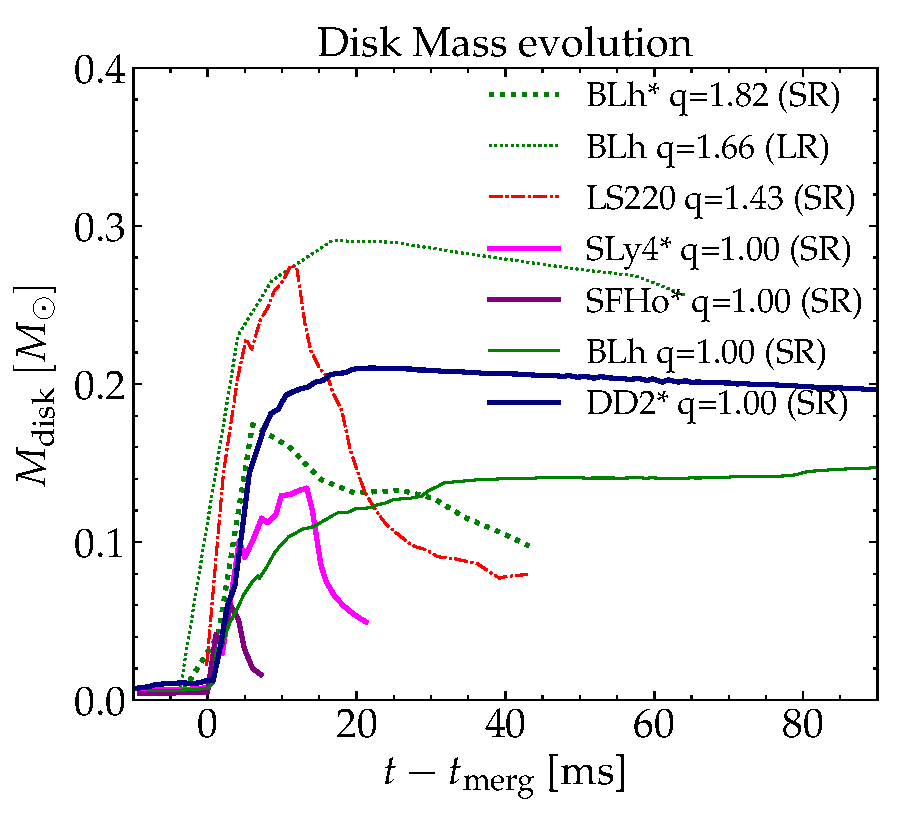
\includegraphics[width=0.49\textwidth]{disk/total_disk_mass_evo.pdf}
    \caption{Time evolution of the total disk mass for a few selected
        short-lived and long-lived cases. The former show a rapid 
        accretion right after disk formation. The plots show
        distinct difference in dynamical evolution after disk formation: accretion onto
        the newly formed BH (short-lived remnants) or accretion onto the NS
        remnant (DD2 $q=1$) with possible continuous mass shedding from the remnant
        into the disk (BLh* $q=1$). Adopted from \citet{Nedora:2020pak}
    } 
    \label{fig:disk_mass_evo}
\end{figure}


\subsection{Binaries with $q\lesssim1.4$}


Binaries with small mass ratio, ($q\lesssim1.4$) produce a \ac{MNS} remnant
that either survives on a dynamical timescale, set by the \ac{NS} rotation, before
collapsing to a \ac{BH}, or a \ac{MNS} that survives till the end of the simulations.
We refer to the former ones as \textit{short-lived} and the latter ones as 
\textit{long-lived} remnants.
Under the first category, fall the \ac{MNS} with relatively soft \ac{EOS}:
LS220 $q=1,1.1,1.2$, SFHo $q=1,1.1,1.4$ and SLy $q=1,1.1,1.4$. 
They collapse within $\sim20$~ms \pmerg. 
The exact time of the collapse however depends on the simulation resolution 
and on the inclusion of subgrid turbulence as was previosly noted by \citet{Radice:2017zta}.

\paragraph{Disk of short-lived remnants}

During the merger, shocks generated at the collisional interface of the \acp{NS} cores,
as well as, tidal torques exerted by the non axisymmetric remnant result in a formation
of the disk. 
Matter, energy and angular momentum are injected into the disk as the spiral density waves 
propagate outwards from the mass-shedding \ac{MNS} remnant 
\citep{Bernuzzi:2015opx,Radice:2018xqa}.
\red{HERE the letter stuff could be added, actually}

Within these waves the fluid reaches highest temperatures, which decrease rapidly, as 
disk expansion and neutrino emission cools the matter. 
In such a high-temperature environment, the electron-positron pair creation is enhanced.
%% [added from Shibata Review paper]
As a result, neutrons can capture positrons $n+e^+p\rightarrow\bar{\nu}_e$.
The average particle energies are large, close to the mass difference between neutron 
and proton. 
In combination with the high $\nu_e$ and $\bar{\nu}_e$ luminosities,
the large number of available positrons leads to an increase 
in the fluid electron fraction, $Y_e$ from that of the initially neutron-rich material
\citep{Qian:1996xt}.
Additionally, a \ac{MNS} is a strong neutrino emitter. The neutrino irradiation of the 
surrounding area alters its composition, and neutrino absorption takes place
$n+\nu_e\rightarrow p + e^{-}$ and $p + \bar{\nu}_e\rightarrow n + e^+$.
This drives the neutron and proton fraction towards equilibrium, and raises the $Y_e$.
\red{paper says: 
    The electron fraction is reset by an initial excess of electron antineutrino emission
    and electron neutrino absorption,}
The entropy per baryon varies between $3$ and $\lesssim 10\,$$k_{B}$/baryon \citep{Perego:2019adq}.
%% ---
If \ac{MNS} remnant collapses to a BH, the main source of neutrinos shuts down and 
the inner part of the disk is rapidly accreted. 
The disk then approaches quasi-steady state, Fig.~\ref{fig:disk_mass_evo}, with 
axisymmetric, approximately Keplerian profile.
The inner part of the resulted disk, at densities $\rho\sim10^{13}$~\gcm, 
is relatively hot, $T\sim10\,$ MeV, but neutron-rich $Y_e\sim0.1$, as it was shielded 
from the neutrino irradiation. The disk gets progressively colder and proton-rich 
outwards with $Y_e$ reaching $0.4$ at the edges.
%% ---
The disk mass at formation appears to depend on the \ac{NS} \ac{EOS}. Binaries with 
stiffer EOS (larger \ac{NS} radii) produce more massive disk.
\red{[Fitting function]
    The disk mass can be described within the numerical uncertainties by a
    quadratic function of the mass ratio and the reduced tidal
    parameters (see Sec.~\ref{sec:remdisk}).}
Additionally, the disk mass show a dependency on mass ratio. For instance, the most massive disks are formed in LS220 $q=1.43$ and  BLh $q=1.82$ models, where the latter experiences prompt collapse.
%% -- 
The disk accretionon a \ac{BH} removes up to $50\%$ of the disk mass on a timescale tens of milliseconds.


\paragraph{Disk of long-lived remnants}


If the \ac{MNS} is long-lived, the disk has time to complete its formation,
and thus it is more massive and extended \citep{Perego:2019adq}. 
As before, the disk is defined as matter, with $\rho\lesssim10^{13}$~\gcm. 
The disk mass increases with the mass ration and with stiffness of \ac{EOS}.
For instance, for BLh $q=1.00$ model, the disk mass reaches ${\lesssim}0.15\,\Msun$, 
while for DD2 $q=1.00$ model is exceeds ${\sim}0.2\,\Msun$.
For a models with BLh \ac{EOS}, the disk mass increases between $q=1.00$ and 
$q\sim1.4-1.5$ by a $100\%$.
%% ---
The long-term evolution of the disk is driven by its interaction with the \ac{MNS} 
remnant and cooling. 
And while in the case of a \ac{BH} remnant, the only possible interaction is the 
disk accretion onto a \ac{BH}, in case of a \ac{MNS} remnant the picture is more 
complex.
The disk neutrino cooling and gravitational pull from the remnant facilitates the 
accretion. However, generated at shocks, spiral density waves inject 
energy and angular momentum into the disk as well as centrifugally supported 
material (as \ac{MNS} undergoes mass-shedding). This heats up the disk and 
facilitates its expansion. 
In the figure  Fig.~\ref{fig:disk_mass_evo} the quasi-steady state disk accretion
is seen for the DD2 $q=1.00$ model. Meanwhile, in the BLh $q=1.00$ model, the 
mass-shedding by the remnant adds more material into the disk that it is being 
accretted. 
The analysis suggests, that this behaviour is due to two main factors: the 
very high average temperatures of the remnant and the disk achieved by this model, that 
are a consequence of the thermal effects included into the BLh EOS (\red{see sec.EOS}),
and the softness of the EOS, which lead to the strong oscillations of the 
remnant after merger (\red{see sec.DensyModes.}).

The inclusion of the subgrid turbulence smears the mass distribution of disk 
properties. The distributions of electron fraction, entropy per baryon and 
temperature appears broader. A more detailed quantitative analysis would require more 
simulations performed at several resolutions to disentangle the effects 
caused by the subgrid turbulence and by the finite grid \citep{Bernuzzi:2020txg,Radice:2020ids}.

\begin{figure}[t]
    \centering 
    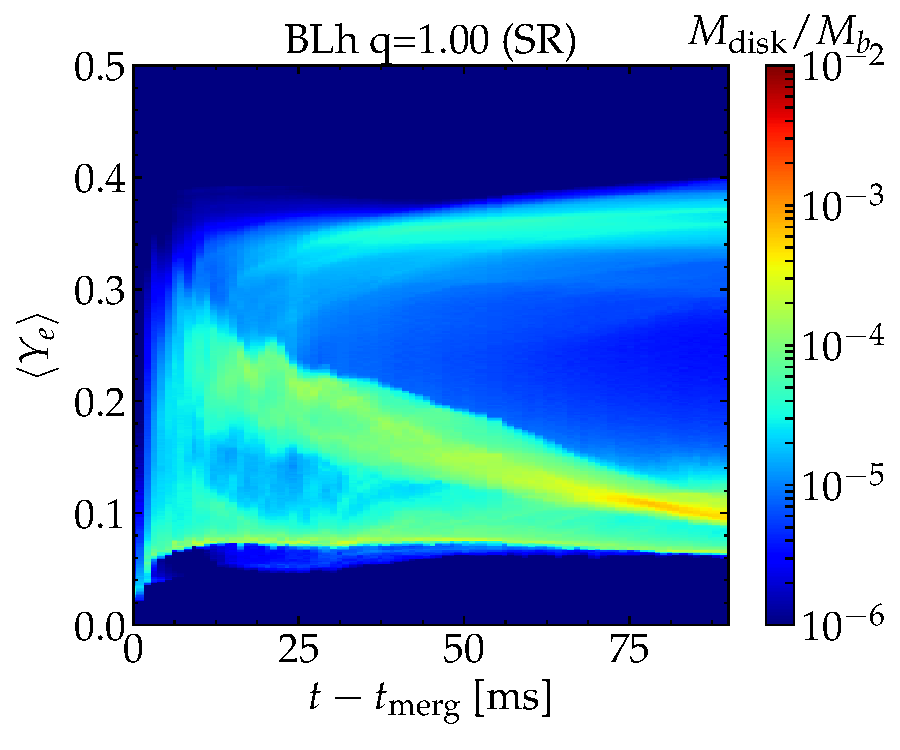
\includegraphics[width=0.49\textwidth]{disk/final_disk_timecorr_blh_q1_Lk.pdf}
    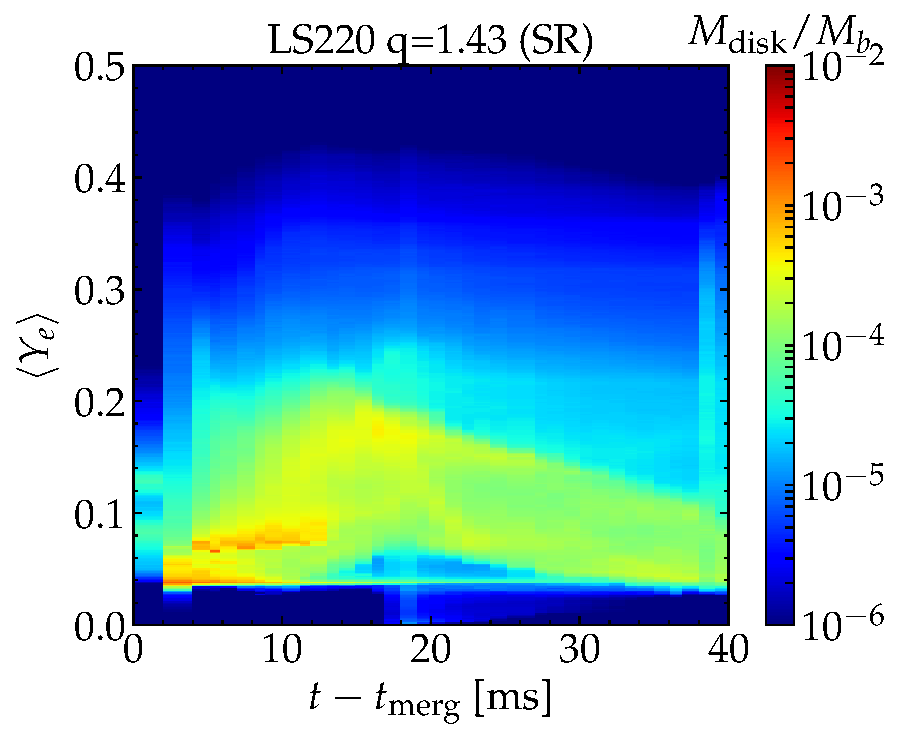
\includegraphics[width=0.49\textwidth]{disk/final_disk_timecorr_ls220_q14_LK.pdf}
    \caption{Evolution of the disk mass-averaged electron fraction with
        time for a long-lived (top) and a short-lived (bottom)
        remnant. The plot shows that with time the bulk of the disk lowers
        its $Y_e$ via cooling, while a small fraction in terms of mass
        gains a high $Y_e$, which relates to the highly 
        irradiated surface of the disk. Adopted from \citet{Nedora:2020pak}.
    }
    \label{fig:total_disk_time_corr_Ye_Blh_q1}
\end{figure}

\paragraph{Evolution of disk properties}

%% Ye evolution
The evolution of the mass-weighted electron fraction for the model
BLh $q=1.00$, the model that is evolved till $\sim 90$~ms after merger, 
is shown on the top panel of Fig.~\ref{fig:total_disk_time_corr_Ye_Blh_q1}.
%% --- 
During the formation, shock and spiral waves raises the disk electron fraction to
$Y_e\sim0.25$. As the disk evolves, the bulk of its mass, shielded from neutrinos, 
(Fig. \ref{fig:slice:heating_hu}, density contours) 
returns to neutron-rich condition with $Y_e\lesssim0.1$. 
The outer part of the disk, however, is subjected to the 
strong neutrino irradiation and reaches $Y_e\sim0.4$ of a timescale of ${\sim}40$~ms.
%% Note that neutrinos in merger remnants decouple at $\rho\sim10^{11}$~$\gccm$ \citep{Endrizzi:2019trv}. 
Notably, the apparent gap in the $Y_e$ distribution if Fig.~\ref{fig:total_disk_time_corr_Ye_Blh_q1} at $\langle Y_e \rangle \simeq 0.15$ 
might not be of physical origin, but an artifact from the neutrino M0 scheme, 
that assumes neutrinos propagate along the radial directions
(see sec.NEUt.M0.SCHEME), that is not well suited for capturing the 
neutrino emission and reabsorption from the disk midplane.
%% ---
In case of a short-lived model LS220 $q=1.43$ model 
(lower panel of the Fig.~\ref{fig:total_disk_time_corr_Ye_Blh_q1})
the average electron fraction is lower, as there is no strong neutrino 
emitter. Additionally, the outskirts of the more compact disk remain 
at low electron fraction as the neutrino emitted by the disk itself 
are the only source of neutrinos. 

\paragraph{Mass ejection on a long timescale}

As the disk expands and cools, the recombination of nucleons into 
alpha particles starts to take place.
The energy, released in recombination, might be sufficient for the outermost 
layers to become unbound, generating an outflow 
\citep{Beloborodov:2008nx,Lee:2009uc,Fernandez:2013tya}.
This processes however are expected to take place on a longer timescales,
that those that are simulated here.
On the $\sim100$~ms timescale, the outflows are driven by the neutrino heating, 
above the remnant, the so-called neutrino-driven wind 
(\nwind; \citealt{Dessart:2008zd,Perego:2014fma,Just:2014fka}),
and by the dynamical interactions between the \ac{MNS} 
remnant and the disk, the \swind{} \citep{Nedora:2019jhl}.
%% ---
We discuss the properties of the \nwind{} found in our simulations
in the section \red{sec.Ejecta.NuWind} and the properties of the 
\swind{} in the \red{sec.Ejecta.SWIND}.
%The \swind{} can have a mass up to
%a few $10^{-2}\,\Mo$ and velocities ${\sim}0.2$~c. The ejecta
%have electron fraction typically larger than ${\sim} 0.25$ since they are 
%partially reprocessed by hydrodynamic shocks in the expanding arms. 
%The \nwind{} is driven by neutrino heating above the remnant. It generates outflows
%with smaller masses ${\sim} 10^{-4}M_{\odot}$ and larger $Y_e$
%than the \swind{}. 
%Differently from \swind{} the mass flux of the \nwind{} in our simulations subsides 
%before the end of out simulations, due to rapid baryon loading of the 
%polar region.
%The \swind{} will be discussed in detail in Sec.~\ref{sec:spiralw}.
The effects of these outflows on the dynamical evolution of the remnant 
lies in the amount of mass and energy they can remove from the system.
Specifically, the \nwind{} have a typical mass of ${\sim} 10^{-4}\Msun$, 
while the \swind{} could remove $10^{-2}\,\Msun$ on a timescale of a $\sim100$~ms.

\begin{figure}[t]
    \centering 
    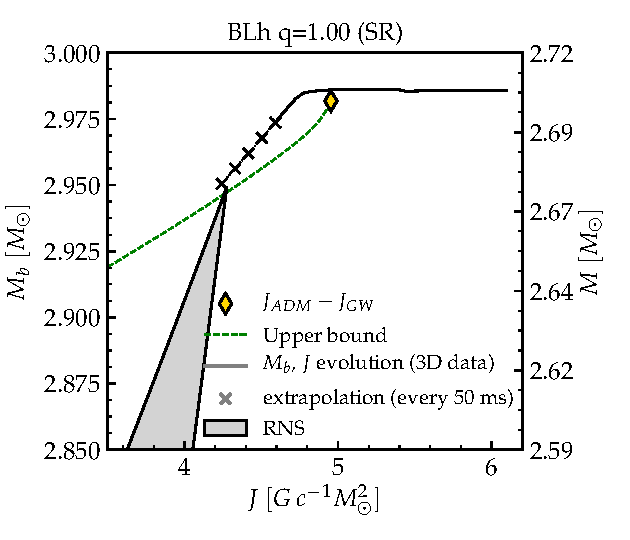
\includegraphics[width=0.49\textwidth]{ejecta_sec/secular_j_mb_RNS_blh.pdf}
    \caption{Baryon mass vs angular momentum diagram for the BLh $q=1$ remnant.
        The colored diamond marks the baryonic mass and angular momentum at the end
        of the dynamical gravitational-wave dominated phase.
        After the GW phase, the evolution is driven by the massive outflows.
        The solid black line is the $M_b$ and $J$ estimated from the 3D data
        integrals under the assumption of axisymmetry.
        The green dashed line is a conservative estimate
        of the mass ejection and a possible trajectory for the viscous
        evolution as estimated in \citet{Radice:2018xqa}. The crosses are
        a linear extrapolation in time of the solid black line. The gray
        shaded region is the region of stability of rigidly rotating NS equilibria.
        Adopted from \cite{Nedora:2020pak}
    }
    \label{fig:total_j_mb_rns_blh}
\end{figure}

To understand the remnant evolution on the timescales longer then the ones 
present here, requires ab-initio \ac{NR} simulations in $(3+1)D$ with compete physics.

Here we consider a BLh $q=1.00$ simulation, one of the longest runs we have performed.
After the merger, the \ac{MNS} remnant is born. With respect to the zero-temperature 
beta-equilibrium \ac{NS} configurations, the BLh $q=1.00$ 
remnant has an excess in baryon mass.
In the figure~\ref{fig:total_j_mb_rns_blh} we show the evolution of the 
total baryon mass, $M_b$, and total angular momentum, $J$, of the remnant.
As the total baryon mass is conserved (if there is no outflow), the early evolution 
of the remnant proceeds with $M_b=\text{const}$. The angular momentum is however 
lost by the remnant to emission of \acp{GW}. 
We evaluate the amount of angular momentum lost to \acp{GW} following the 
\citet{Damour:2011fu,Bernuzzi:2012ci,Bernuzzi:2015rla}.
\red{This has to be defined and noted that we use $\sim20$~ms postmerger mark
    and how exactly we compute all of it, the David's script
}
Substruct it from the initial data \ac{ADM} angular momentum we obtain the value 
that is left to the system after the \ac{GW} phase 
(the yellow marker on the Fig.~\ref{fig:total_j_mb_rns_blh}).
%% ---
Notably, after the \ac{GW} phase, the remnant still has an excess in angular momentum
in comparison with the rigidly rotating \ac{NS} configurations with the same baryon mass 
(gray triangular region in Fig.~\ref{fig:total_j_mb_rns_blh}).
We observe the same situation across all models \citep{Zappa:2017xba,Radice:2018xqa}.
\gray{
    On the angular momentum estimation:
    The radiated angular momentum (as well as energy) are computed from the 
    multipole loments $N_{lm}$ for the \ac{NR} complex "news function" at infinity. 
    The $J_{z;\text{rad}}(t)$ is computed as \citep{Damour:2011fu} 
    \begin{equation}
    \Delta J_{z\text{rad}}(t) \frac{1}{16}\sum_{l,m}^{l_{max}}\int_{t_0}^{t} dt' m \mathcal{L}[h_{lm}(t')(N_{lm}(t'))^*],
    \end{equation}
    where $h_{lm}$ is the multipolar metric waveform, 
    $N_{lm}(t) = dh_{lm}(t) / dt$, the news function, and $l_{max}=8$.
    The $J$ loss is metric dependent ($h$).
    The $h$ (strain???) is computed from $\Psi_4(t) = dN/dt = d^2h/dt^2$ by a 
    frequency-domain integration procedure with a low-frequency cut 
    $\omega_0 = 0.032/(m_1+m_2)$.
}
%% ---
The baryon mass of the remnant also exceeds maximum mass that a rigidly rotating 
equilibria could have.
Such remnant is generally referred to as a hypermassive neutron star (HMNS) following the 
nomenclature introduced for zero-temperature EOS equilibria \acp{NS} \citep{Baumgarte:1999cq}.
Such a remnant is expected to collapse to a BH. 
%% ---
However, a remnant can avoid the collapse by efficiently removing angular momentum
and mass and entering the rigidly rotating equilibria zone. 
%% ---
We compute the angular momentum and baryon mas evolution of the remnant, 
through volume integrals, assuming axisymmetry and evaluating the former using Eq.~\eqref{eq:method:ang_mom}, and the latter using the Eq.~\eqref{eq:method:mdisk}. 
The evolution of these two quantities is depicted with the black solid line if 
Fig.~\eqref{fig:total_j_mb_rns_blh}~\footnote{Note that the angular momentum estimated
    from the GW and from the integral of Eq.~\eqref{eq:method:ang_mom} assuming
    axisymmetry are compatible within the errors made in the latter estimate.
}.
We observed that after the \ac{GW} phase, the remnant continues to evolve, loosing the 
angular momentum together with the baryon mass. This is achieved through massive outflow,
the \swind{}. 
The extrapolation of the final trend of the mass and angular momentum loss shows, that 
if $\approx0.05\,\Msun$ ($\approx40$\% of the final disk at the end of simulation) is 
ejected, the \ac{MNS} remnant would approach the rigidly rotating equilibria region 
at the mass-shedding limit. Extrapolation indicates, that if the ejecta mass flux does 
not change, this would occur on a timescale of $\sim 300$~ms \pmerg{}.
Similar results are obtained with the conservative upper bound estimate on the 
evolution of the long-lived remnant (Eq.~$2$ in \citet{Radice:2018xqa}) (green dashed line in figure).
\red{WHAT the fuck is Keplerian limit, mass-shedding limit and rigidly rotating equilibria}
Additionally, while this simulation included the effects of turbulent viscosity on the
angular momentum transport, the ejecta could be further enhanced by the magnetic stresses 
\citep{Metzger:2006mw,Bucciantini:2011kx,Siegel:2017nub,Fernandez:2018kax,Ciolfi:2020hgg}.

Other simulations also produce a \ac{MNS} remnant with a similar evolutionary path. 
Models with DD2 \ac{EOS} however, are born with an excess in angular momentum, but not in 
baryon mass. They also evolve toward the rigidly rotating equilibria but slower.
Models with $q>1.00$ produce remnants that generally have larger excess in angular momentum 
and mass have how to shed a larger amount of mas to reach equilibrium configuration.
(\red{However we also show that these models tend to have stronger \swind{}, see sec.SPIRAL.WIND})
Overall, we estimate that for models with $q=1.00$ need to shed ${\sim}0.05\Msun$ while 
models with $q\eqsim 1.4$ need to remove $0.2\Msun$ to reach equilibrium configuration.



\section{Mass Ejection}



Tidal interactions and shocks exerted on the \acp{NS} at merger trigger the ejection of material
on the dynamical timescale. This is the \ac{DE} \citep[\eg][]{Hotokezaka:2013b,Bauswein:2013yna,Radice:2016dwd,Radice:2018pdn}. 



\subsection{Dynamical Ejecta}


%% The mechanism behind the dynamical ejecta [radice:2018pnd]
Tidal interactions and shocks exerted on the \acp{NS} at merger trigger the ejection of material
on the dynamical timescale. This is the \ac{DE} \citep[\eg][]{Hotokezaka:2013b,Bauswein:2013yna,Radice:2016dwd,Radice:2018pdn}. 

\red{More on the genral mechanism tidal vs shocked}
The \ac{DE} is evaluated with the geodesic criterion introduced in Sec.~\ref{sec:method:analysis:ejecta}.

Describe shock vs tidal components 

\subsubsection{Overall properties of the \ac{DE}}


The novelty of the set of models discussed in this thesis with respect to the 
previous study by \citet{Radice:2018pdn} is that all models include the neutrino heating via M0 scheme 
(see Sec.\ref{sec:theory:neutrino}) in addition to the neutrino cooling and for most models the effects 
of subgrid turbulence (see Set.\ref{sec:theory:grles}) are included.
Meanwhile, models cover a significantly more narrow range in 
dimensionless tidal deformability, $\tilde{\Lambda}$, and mass ratio, motivated by the \GW{}.

We can qulitativly asses the effects of neutrino heating by comparing the overall properties 
of our model set and that of the \citet{Radice:2018pdn}.
Specifically, the neutrino absorption leads to not only an increase in average electron 
fraction but also to larger total ejected mass and velocity. The latter two would be 
crucial for the non-thermal, kilonova afterglow (see Sec.\red{sec:KilonovaAfterglow}).

The mass averaged over the simulations from Tab.~\ref{tab:sim} is 
$\overline{\amd} = (3.442 \pm 2.495)\times 10^{-3}\,M_{\odot}$ (where
hereafter we report also the standard deviation), while the same
quantity calculated for data of \cite{Radice:2018pdn} 
is $\overline{\md} = (1.352\pm 1.250)\times 10^{-3}\,\Msun$.
The mass-averaged terminal velocity of the dynamical ejecta 
ranges between $0.1$c and $0.3$c, and in a good agreement with 
\cite{Radice:2018pdn}.
The mass-averaged velocity, averaged over all the simulations, is 
$\overline{\avd} = (0.172\pm0.038)\,{\text{c}}$.

We find that in our set of models, there is a correlation of $\avd$ with the tidal parameter 
$\tilde{\Lambda}$: the higher the $\tilde{\Lambda}$ the lower the $\avd$.
This can be understood from the general mechanism of the \ac{DE},
that tells in mergers of binaries with $q=1.00$, the shocked component of the ejecta 
is the dominant. The strength of shocks increases as the \acp{NS} become more compact 
(with decreasing $\tilde{\Lambda}$) and hence collide at higher velocities~\footnote{Note that in the definition of prompt collapse we adopted, there is no shocked ejecta.}.
%% ---
For binaries with high mass ration, however, the tidal component of the \ac{DE} is dominant. 
The velocity of the latter also is smaller for larger $\tilde{\Lambda}$, as stars collide 
at slower velocities due to their larger radii. 
%% ---
The mass-averaged electron fraction, $\ayd$, of our models lies the range $(0.1, 0.3)$
with an averaged value among all models $\overline{\ayd} = 0.175 \pm 0.063$.
Notably, the \citet{Radice:2018pdn} reported a more narrow range, $(0.1, 0.2)$.
This is a clear effect of the neutrino absorption included in our models, that elevates 
the everal electron fraction of the \ac{DE} as it is being irradiated by neutrinos 
during the merger.
Notably, the $\ayd$ of our models is close to those obtained with M1 
scheme of \citet{Sekiguchi:2016bjd} and \citet{Vincent:2019kor}.
%% ---
The effect of subgrid turbulence on the dynamical ejecta properties however,
found rather week and comparible to the effects of finite grid distritization 
\citep{Bernuzzi:2020txg,Radice:2020ids}.

We find that the properties of the \ac{DE} depends on the \mr{} and on the 
\ac{EOS} softness that can be parameterized with $\tilde{\Lambda}$. 
We investigate in detail the statistical properties of our set of models as well as 
other \ac{NR} \ac{BNS} data sets available in the literature in 
section \ref{sec:ejecta_disk_statisitcs}.





\subsection{Fast tail of the dynamical ejecta}

%\begin{figure}[t]
%    \centering 
%    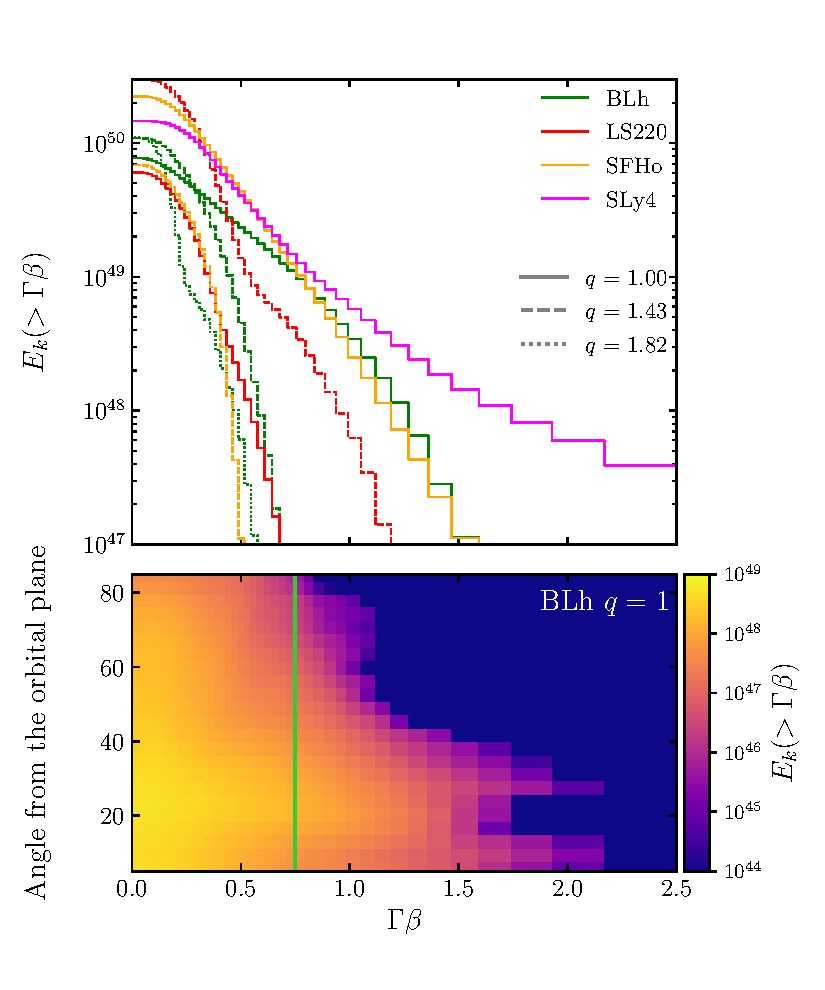
\includegraphics[width=0.49\textwidth]{./figs/kinetic_energy_struct_models.pdf}
%    \caption{
%        Total kinetic energy distribution for a selected set of models (\textit{top panel}) 
%        and angular distribution of kinetic energy for a BLh $q=1.00$ model (\textit{bottom panel}).
%        %% Also shown as a solid black line is the slow quasi-spherical model of \cite{Mooley:2017enz}.
%        The vertical light green line marks the $\upsilon_{\text{ej}}=0.6$.
%        The top panel shows that equal mass models have a more extend high energy tail,
%        while the bottom panel shows that the angular distribution of the ejecta is not 
%        uniform.
%        \red{Adopted from Nedora et al. (2021)}
%    } 
%    \label{fig:ejecta_vel_hist}
%\end{figure}
%
%The velocity distribution of \ac{DE} was found to include a very fast, 
%$\upsilon_{\text{ej}}\geq0.6$~c tail
%\cite{Piran:2012wd,Hotokezaka:2013b,Kyutoku:2012fv,Ishii:2018yjg,Hotokezaka:2018gmo,Radice:2018pdn}.
%%% ---
%The total mass of this tail was found to be dependent on the
%binary parameters and solution resolution,
%with an average $\sim 10^{-6}-10^{-5} M_{\odot}$.
%%% ---
%With respect to the fast tail origin, it can be divided into two main components 
%\citep{Radice:2018pdn}.
%The early component, that comprises the ejecta that is generated at the collisional interface 
%of two \acp{NS} of similar mass and directed primarily along the binary axes.
%And the late component that consist of matter that driven by the shock breakout from the ejecta 
%after the core bounce and confined mostly to the binary plane. 
%
%Among the simulations listed in \ref{tab:sim}, we select \red{XX} simulations 
%performed at standard resolution, and for which fast ejecta is found.
%%% ---
%Here we extract ejecta properties at the detector located at 
%$R=300G/c^2M_{\odot}\approxeq443$~km, from the merger, in agreement with \citet{Radice:2018pdn}.
%
%The mean value of the fast tail mass is
%
%\be\label{eq:ejecta:dyn:avg:M}
%\red{ \overline{\amd}(\upsilon>0.6) = (2.50 \pm 4.23)\times 10^{-5}M_{\odot}\ , }
%\ee
%
%where the standard deviation is also reported as an error.


%% ------------------ 
%% Note that the geodesic criterion above neglects the fluid's pressure and might
%% underestimate the ejecta mass. The Bernoulli criterion assumes that the (test
%% fluid) flow is stationary, so that there is a pressure gradient that can
%% further push the ejecta.  We find that both criteria predict dynamical
%% ejecta masses that are practically indistiguishable and well within the numerical uncertainties \citep{Bernuzzi:2020txg} if applied to extraction spheres at large coordinate radii; 
%% differences between the two criteria are instead present if they are applied to
%% matter volumes \citep[cf.][]{Kastaun:2014fna}.


\subsection{\swind{}}
\label{sec:spiralw}

\begin{figure*}[t]
    \centering 
    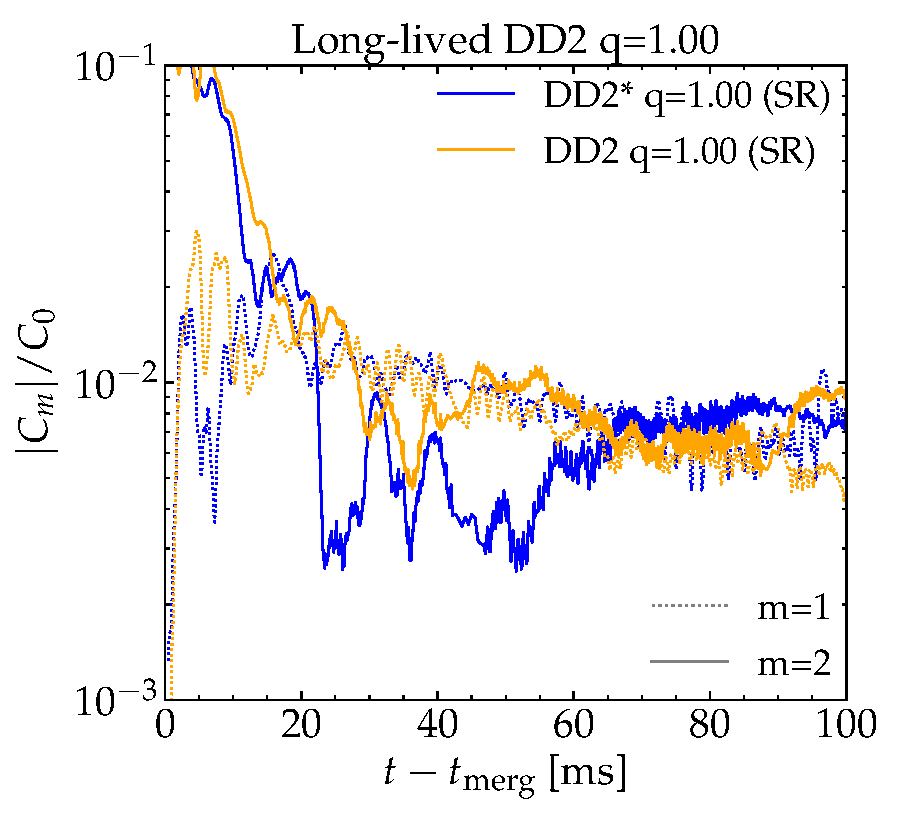
\includegraphics[width=0.49\textwidth]{remnant/dens_modes/modes_rho_dd2.pdf}
    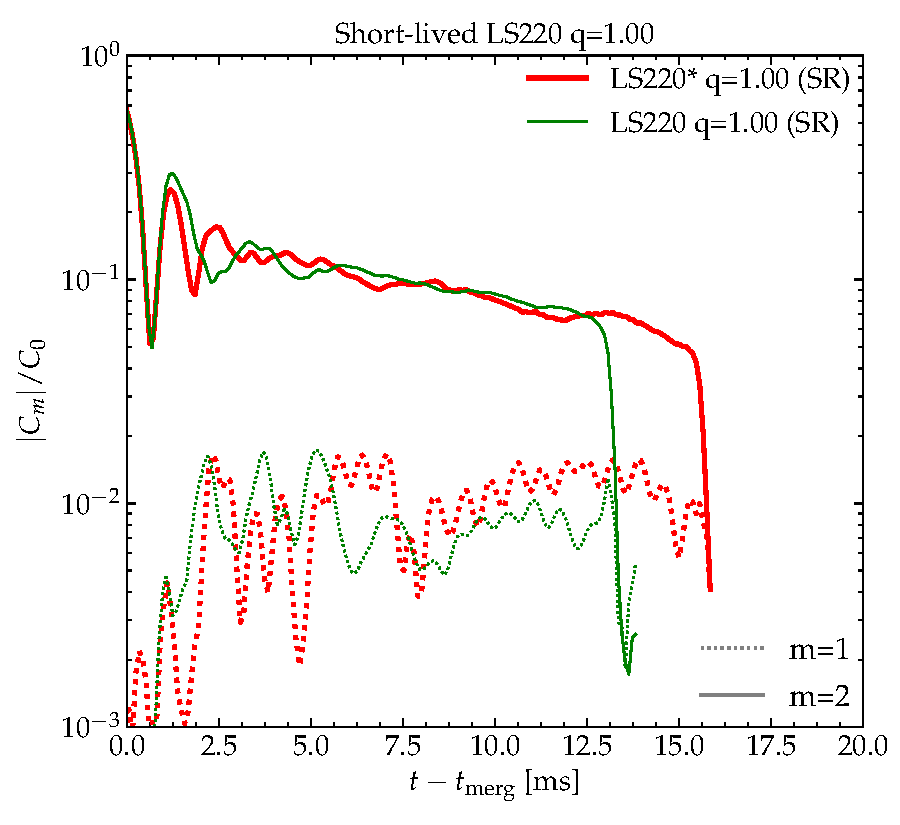
\includegraphics[width=0.49\textwidth]{remnant/dens_modes/modes_rho_ls220.pdf}
    \caption{Modes analysis for exemplary equal-mass long-live and short-lived
        remnants. The evolution of the $m=2$ and the $m=1$ monitored by
        Eq.~\eqref{eq:modes} is shown for the DD2 and LS220 remnant with and
        without turbulent viscosity. The $m=2$ mode in the long-lived
        remnant is strongly damped by the emission of gravitational
        radiation and becomes comparable to the $m=1$ mode on a timescale of
        ${\gtrsim}20\,$ms. Turbulent viscosity sustain the $m=2$ mode for
        a longer period. The $m=2$ mode is instead dominant to collapse in
        the short-lived remnant.
        (Adopted from \cite{Nedora:2020pak})
    }
    \label{fig:dens_modes}
\end{figure*}

Here we discuss the dynamics of spiral waves and the associated outflow, the \ac{SWW}.


\subsubsection{Remnant \& disk dynamics}


The hydrodynamical modes of the \ac{MNS} remnant are computed following the 
method described in Sec.\ref{sec:method:HDmodes}. 
The mode analysis is shown in the Fig.\ref{fig:dens_modes} for two representative 
simulations, the short-lived LS220 $q=1.00$ and the long-lived DD2 $q=1.00$.
The newly born \ac{MNS} remnant is not axisymmetric, displaying characteristic 
spiral arms, extending outwards from the shock interface of the collided cores 
\citep{Shibata:1999wm,Shibata:2006nm,Bernuzzi:2013rza,Kastaun:2014fna,East:2015vix,Paschalidis:2015mla,Radice:2016gym,Lehner:2016wjg}.
The bar-shaped, $m=2$ modes is the dominant one early in \pmerg{}, while the 
one-armed spiral $m=1$ modes stars to dominate in the late evolution 
\citep{East:2015vix,Paschalidis:2015mla,Radice:2016gym,Lehner:2016wjg,Bernuzzi:2013rza,Kastaun:2014fna}.
Indeed, the $m=2$ mode remains the dominant one until $\sim15-20$~ms \pmerg{}. 
After that, the LS220 $q=1.00$ model forms a \ac{BH}. 
In the DD2 $q=1.00$ model, however, the $m=1$ mode becomes comparable with $m=1$ 
throughout the remainder of the evolution, while the $m=2$ mode efficiently dissipates 
through \ac{GW} emission \citep{Bernuzzi:2015opx,Radice:2016gym}.
%% ---
We find that the magnitude of the $m=1$ mode increases with the binary \mr{}.
For instance the largest $C_{m=1}$ are found in BLh $q=1.43$ and LS220 $q=1.22$.
Stronger $m=1$ leads to more large \ac{SWW} mass flux.
The dependency of the $C_{m=2}$ on \mr{} however is not clear. 
This is in agreement with what reported by \citet{Lehner:2016wjg}.

Formation of the spiral arms is a generic hydrodynamic effect, that was identified 
in the \ac{NR} simulations with polytropic \ac{EOS} 
\citep{Bernuzzi:2013rza,Radice:2016gym}.
However, the evolution of these arms and quantitative behaviour of hydrodynamic
modes depends on the physics input. 
In the Fig.~\ref{fig:dens_modes} we show that the turbulent viscosity in the 
DD2 $q=1.00$ remnant stabilizes the $m=2$ mode, enhancing the angular momentum 
transport into the disk.
The $m=2$ mode, however, remains largely unaffected by the turbulent viscosity.
Similarly, the models' evolution in the LS220 $q=1.00$ is too short, for the 
subgrid turbulence to become important.

We compute the angular momentum of the \ac{MNS} remnant following the method,
discussed in Sec.\ref{sec:method:angmom}, where the remnant is distinguished 
from the disk on the basis of the rest mass density $\rho=10^{13}$~\gcm{} 
(see Sec.\ref{sec:method:diskdef}).
We find that for a long-lived rmnant 
on a timescale of $\sim20$~ms, about half of the total angular momentum 
of the \ac{MNS} remnant is transferred into the disk. 
%% [ from shibata review ]
This is a consequence of the fact that the remnant \ac{MNS} is strongly deformed 
after merger and gravitational torque on the surrounding matter, 
that allows for a rapid angular momentum transport.
%% ---
After, the remnant settles on quasi-stationary evolution path 
(see Sec.~\ref{sec:bns_dynsmics_overview}).

Following the disk and remnant mass evolution we observe, that the spiral 
density modes inject ${\sim}0.1-0.4\,\Msun$ of baryon mass into the disk during the 
first ${\sim}20$ms. 
The mass injection appears to be stronger for stiffer \acp{EOS}. 
With respect to the \mr{}, the higher $q$ binaries form a larger disc 
(see BLh* $q=1.82$ and LS220* $q=1.43$ on the Fig.~\ref{fig:disk_mass_evo}).

\begin{figure}[t]
    \centering 
    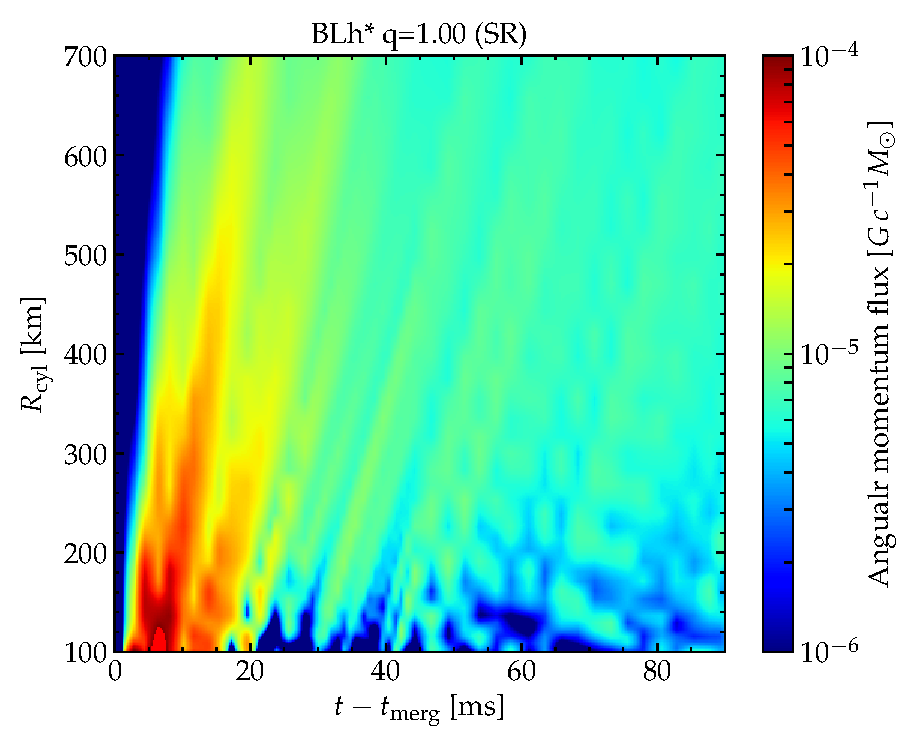
\includegraphics[width=0.49\textwidth]{remnant/evol_jflux_2d_BLh_M13651365_M0_SR_R1.pdf}
    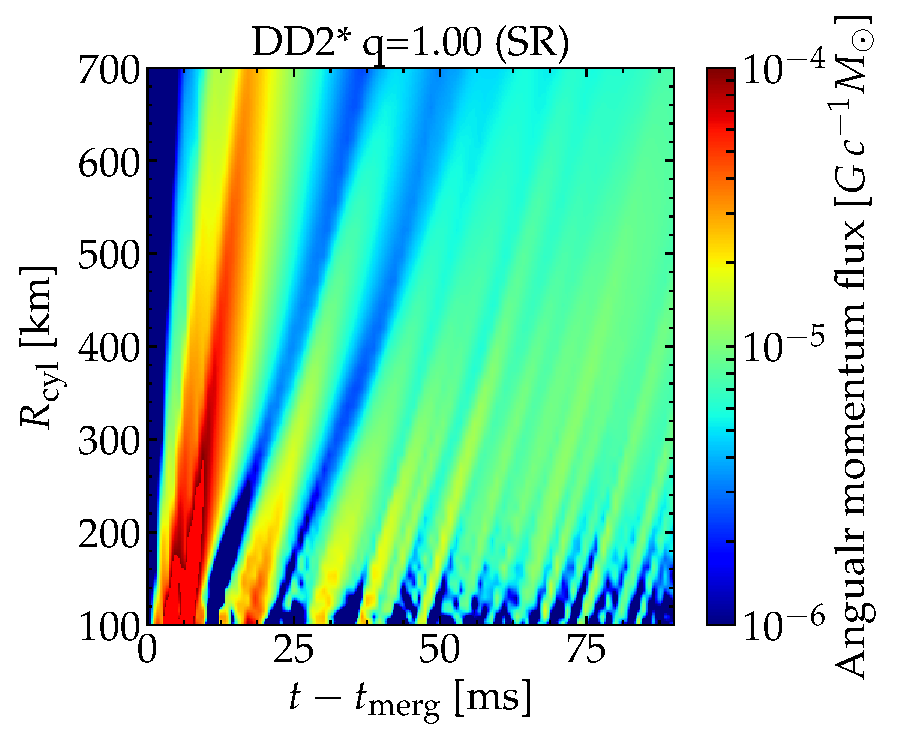
\includegraphics[width=0.49\textwidth]{remnant/evol_jflux_2d_DD2_M13641364_M0_SR_R1.pdf}
    \caption{Angular momentum flux through consecutive cylindrical
        surfaces identified by cylindrical radii from $R_{\text{cyl}}=100$ to $R_{\text{cyl}}=500$. The
        plot shows the angular momentum transport into the disk.
        Adapted from \citet{Nedora:2020pak}
    }
    \label{fig:disk_ang_mom_flux_map_blh_q1}
\end{figure}

In the Fig.~\ref{fig:disk_ang_mom_flux_map_blh_q1} we show how the 
angular momentum is being transported from the \ac{MNS} remnant into the disk
in two long-lived models with turbulent viscosity, DD2* $q=1.00$ and BLh $q=1.00$.
The angular momentum is transported via spiral waves that correspond do the 
hydrodynamic models, $m=1$ and $m=2$ discussed above.
We observer, that in the model with more stiff DD2 \ac{EOS},
the fist wave is stronger. Notably, the DD2* $q=1.00$ model 
also has a more massive disk.
%% --- 
Further, the evolution of the disk-remnant interactions 
after $\sim20$~ms \pmerg{} is different for two models. 
While the model with DD2 \ac{EOS} stops shedding mass into 
its disk and starts slowly accreting, the model with BLh \ac{EOS} continues to shed mass into the disk
(see Fig.~\ref{fig:disk_mass_evo} and discussion in
Sec.~\ref{sec:bns_dynsmics_overview})
The latter is caused by the strong angular momentum flux \red{actually the plot shows, that it is not}, emanating 
from the \ac{MNS} remnant and by the larger temperatures, 
that reached in the model with the BLh \ac{EOS}.
Larger temperatures leads to lower rotational frequency 
at which the mass shedding occurs \citep{Kaplan:2013wra}. 

The subgrid turbulence enhances the angular momentum transport. However more simulations of long-lived 
\ac{MNS} remnants are needed to asses the effects of the 
subgrid turbulence and \mr{} systematically. 

\begin{figure}[t]
    \centering 
    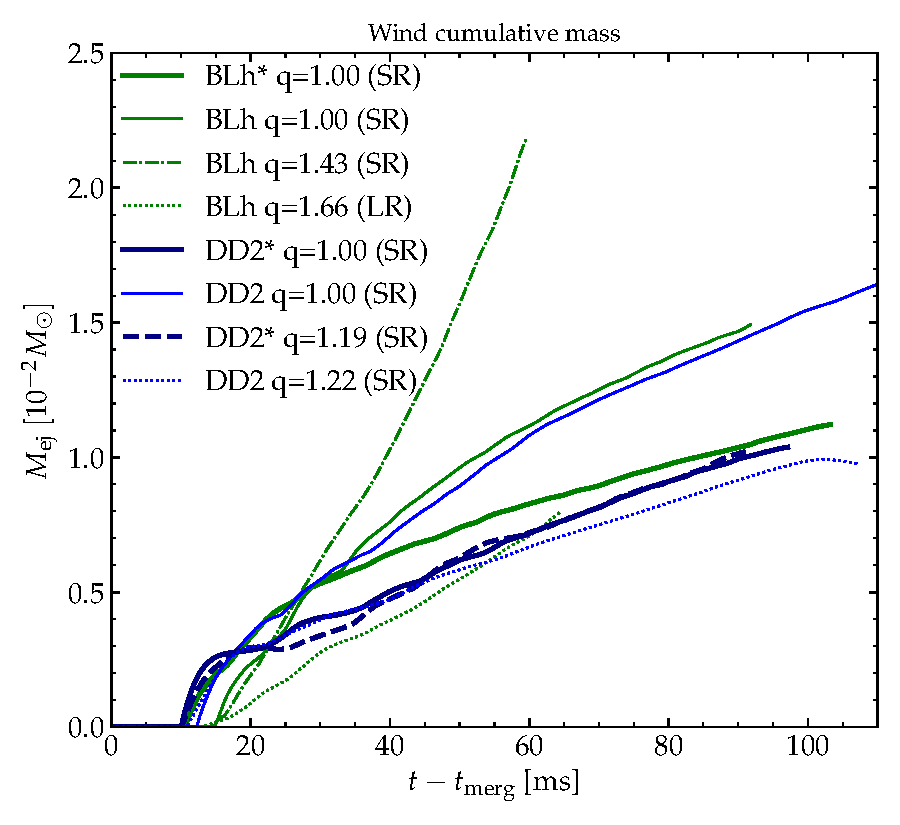
\includegraphics[width=0.50\textwidth]{ejecta_postdyn/wind_mass_flux.pdf}
    \caption{Cumulative mass of the \swind{} from long-lived
        remnants. The wind persists on timescales of $\O(100)\,$~ms with
        mass fluxes ${\sim}0.33-1.23\,\Msun/s$.
        Adapted from \citet{Nedora:2020pak}.
    }
    \label{fig:mej:bern}
\end{figure}

\begin{figure*}[t]
    \centering 
    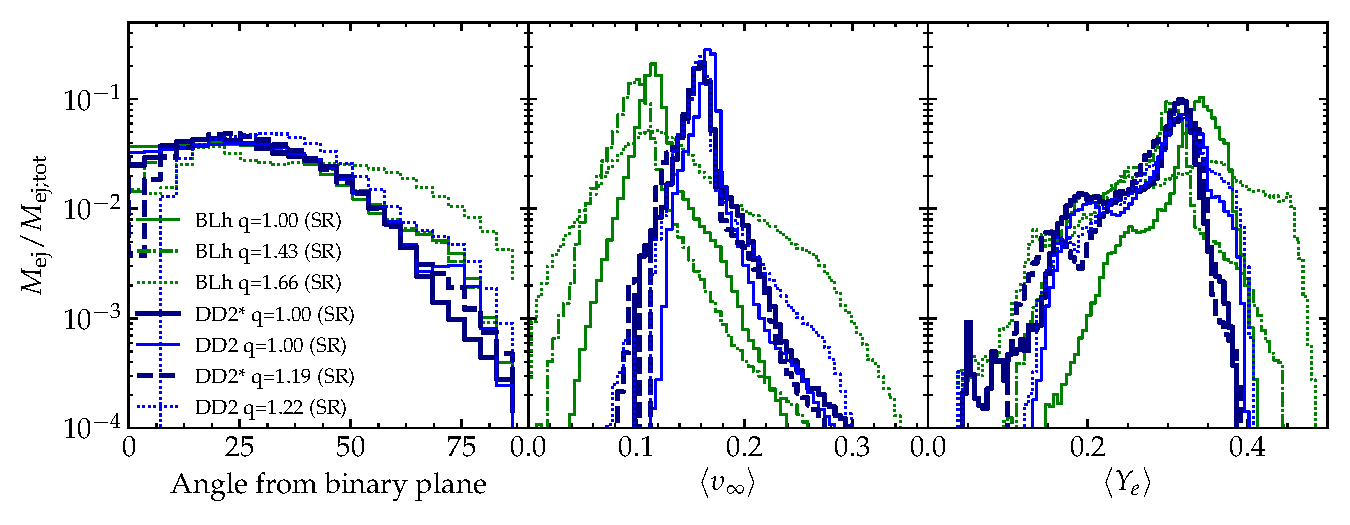
\includegraphics[width=0.99\textwidth]{ejecta_postdyn/wind_hists_shared.pdf}
    \caption{Mass-averaged histograms of the \swind{} for a selected
        subset of long-lived remnant. From left to right: ejecta angular
        distribution, ejecta terminal velocity and electron
        fraction. Remnants from more asymmetric binaries produce winds
        with broader angular distribution.
        The \swind{} from the DD2 EOS remnants has larger velocities
        then the winds from the softer BLh EOS. The electron fraction
        peaks at ${\sim}0.3$ and it is distributed from $0.1$ to $0.4$.
        Adapted from \citet{Nedora:2020pak}.
    }
    %
    \label{fig:ejecta:bern:hist}
\end{figure*}

%% --------------------------------
%% TAB WIND SUMMARY
\begin{sidewaystable}
%\begin{table*}[t]
  \centering
  \captionsetup{width=1.0\linewidth}
  \caption{%
    Summary table of the \swind{} properties of long-lived remnants. The columns contain
    the following information, starting from the left. Equation of
    state, mass-ratio, available resolutions,
    inclusion of subgrid turbulence, time of the
    simulation end, mass of the
    \swind{}, mass-loss rate via \swind, mass-averaged electron fracton, terminal
    velocity and, finally, RMS angle for \swind{}. For these four
    quantities we give the mean value among the resolutions and
    one-sigma deviations. For binaries for which only one
    resolution is present, the error is assumed to be $20\%$ of the value.
    (Adapted from \cite{Nedora:2020pak}).
    }
  \label{tab:spiralwavewind}
  \begin{tabular}{c c c c c c c c c c}
    \hline\hline
    EOS & $q$ & Resolution & GRLES & $t_{\text{end}}$ & $\amw$ & $\amw/\Delta t$ & $\ayw$ & $\avw$ & $\langle \theta_{\text{ej}}^{\text{w}} \rangle$ \\
    &   &   &   & [ms] & $[10^{-2} M_{\odot}]$ & $[M_{\odot}/s]$ &   & $[c]$ &   \\ 
    \hline
    \hline
    BLh & 1.00 & \texttt{SR HR LR} & \cmark & $43.3$ $91.8$ $23.1$ & $0.39^{+0.07} _{-0.07} $ & $0.70^{+0.32} _{-0.32} $ & $0.31^{+0.01} _{-0.01} $ & $0.12^{+0.01} _{-0.01} $ & $27.06^{+2.61} _{-2.61} $ \\
    BLh & 1.00 & \texttt{SR} & \xmark & $ $ $103.2$ $ $ & $1.12^{+0.57} _{-0.57} $ & $1.07^{+0.21} _{-0.21} $ & $0.34^{+0.01} _{-0.01} $ & $0.12^{+0.02} _{-0.02} $ & $15.72^{+2.00} _{-2.00} $ \\
    \hline
    BLh & 1.18 & \texttt{LR} & \cmark & $69.4$ $ $ $ $ & $1.28^{+0.64} _{-0.64} $ & $1.23^{+0.25} _{-0.25} $ & $0.33^{+0.01} _{-0.01} $ & $0.11^{+0.02} _{-0.02} $ & $14.98^{+2.00} _{-2.00} $ \\
    \hline
    BLh & 1.43 & \texttt{LR SR} & \cmark & $35.1$ $59.6$ $ $ & $0.75^{+0.18} _{-0.18} $ & $1.06^{+0.67} _{-0.67} $ & $0.27^{+0.01} _{-0.01} $ & $0.09^{+0.01} _{-0.01} $ & $19.43^{+2.22} _{-2.22} $ \\
    \hline
    BLh & 1.54 & \texttt{LR} & \cmark & $45.8$ $ $ $ $ & $0.63^{+0.32} _{-0.32} $ & $0.44^{+0.09} _{-0.09} $ & $0.32^{+0.01} _{-0.01} $ & $0.10^{+0.02} _{-0.02} $ & $21.46^{+2.00} _{-2.00} $ \\
    \hline
    BLh & 1.66 & \texttt{LR SR} & \cmark & $64.6$ $20.1$ $ $ & $0.12^{+0.09} _{-0.09} $ & $0.37^{+0.34} _{-0.34} $ & $0.33^{+0.05} _{-0.05} $ & $0.13^{+0.01} _{-0.01} $ & $52.08^{+20.89} _{-20.89} $ \\
    \hline
    \hline
    DD2 & 1.00 & \texttt{LR SR HR} & \cmark & $123.0$ $113.0$ $74.4$ & $1.25^{+0.14} _{-0.14} $ & $1.30^{+0.19} _{-0.19} $ & $0.30^{+0.01} _{-0.01} $ & $0.17^{+0.00} _{-0.00} $ & $14.88^{+0.87} _{-0.87} $ \\
    \hline
    DD2 & 1.20 & \texttt{LR SR HR} & \xmark & $37.3$ $91.0$ $55.2$ & $0.48^{+0.09} _{-0.09} $ & $0.74^{+0.24} _{-0.24} $ & $0.26^{+0.01} _{-0.01} $ & $0.15^{+0.00} _{-0.00} $ & $24.54^{+2.23} _{-2.23} $ \\
    \hline
    DD2 & 1.43 & \texttt{LR SR} & \cmark & $37.7$ $62.0$ $ $ & $0.60^{+0.02} _{-0.02} $ & $0.51^{+0.06} _{-0.06} $ & $0.23^{+0.12} _{-0.12} $ & $0.16^{+0.00} _{-0.00} $ & $21.74^{+0.03} _{-0.03} $ \\
    \hline
    \hline
    SFHo & 1.43 & \texttt{SR} & \cmark & $ $ $46.5$ $ $ & $0.58^{+0.30} _{-0.30} $ & $0.43^{+0.09} _{-0.09} $ & $0.31^{+0.01} _{-0.01} $ & $0.17^{+0.02} _{-0.02} $ & $22.67^{+2.00} _{-2.00} $ \\
    \hline
    \hline
    SLy4 & 1.43 & \texttt{SR} & \cmark & $ $ $40.3$ $ $ & $0.53^{+0.27} _{-0.27} $ & $0.38^{+0.08} _{-0.08} $ & $0.29^{+0.01} _{-0.01} $ & $0.18^{+0.02} _{-0.02} $ & $23.52^{+2.00} _{-2.00} $ \\
    \hline\hline
\end{tabular}
%\end{table*}
\end{sidewaystable}

%% --------------------------------


\subsubsection{Properties of the \swind{}}


Density waves, propagating outwards through the disk induce the outflow, the \ac{SWW} 
\citep{Nedora:2019jhl}.

\red{HERE THE LETTER STUFF COULD GO}

The \ac{SWW} is estimated following the Bernoulli criterion as described in 
the Sec.~\ref{ec:method:analysis}. 
We start to follow the \ac{SWW} after the \ac{DE} has saturated. 

We report the overall properties of the \ac{SWW} for all the models with the 
long-lived \ac{MNS} remnant that were also evolved for a sufficiently long time 
in the Tab.~\ref{tab:spiralwavewind}. 
The time evolution of the total mass of the \ac{SWW} is shown in the Fig.~\ref{fig:mej:bern}.
We observe that in all simulations \acp{SWW} persists till end without saturation.
This is because the outflow is driven by the angular momentum and mass transport 
induced by the dynamical instabilities in the remnant, the $m=1,2$ modes, discussed 
above. And as the $m=1$ modes are not efficiently damped \citep{Paschalidis:2015mla,Radice:2016gym,Lehner:2016wjg,East:2016zvv},
the \ac{SWW} could theoretically continue until the system collapses to a \ac{BH} 
or reaches the equilibrium (Sec.~\ref{sec:bns_dynsmics_overview}).

The strongest \ac{SWW} is found in binaries with $q>1$, such as 
$q=1.67$ and LS220 $q=\red{1.4}$. 
With the mass-loss rate ${\sim}0.5\, \Msun/{\text{s}}$, these models can eject 
${\sim}0.02\,\Msun$ within ${\sim}50$~ms of \pmerg{} evolution.
We find that as the \ac{EOS} becomes softer, lower \mr{} is needed to achieve high 
mass flux. For instance, the \ac{SWW} mass flux for BLh* $q=1.66$ is achieved by the 
model LS220* with $q=1.22$. 
A possible explanation for this is that the models with softer \ac{EOS} have stronger 
$m=1$ modes in the remnant (see Sec. \ref{sec:remdisk}).
When \ac{MNS} remnant collapses to a \ac{BH} and the mechanism that injects angular 
momentum into the disk shuts down, the \ac{SWW} mass flux subsides. 
Thus, the total ejected mass via \ac{SWW} is directly related  o the lifetime of the 
\ac{MNS} remnant, an addition to the binary parameters, \ac{EOS} and \mr{}.

The \ac{SWW} mass flux depends on the disk configuration, as more extended disks 
have outer layers that are less gravitationally bound. In turn, the disk 
configuration is dependent on the thermal effects. Higher temperature leads to 
stronger thermal pressure that increases the disk size. 
However, the dependency of the \ac{SWW} mass flux on the stiffness of the \ac{EOS} 
appears to be stronger, as the stiffer \ac{EOS} leads to a more massive disk 
(Sec.~\ref{sec:overview}). More simulations with longer postmerger evolution are needed 
to make a quantitative assessment. 
Overall the \swind{} from the long-lived remnant has a mass flux $\geq 0.4\, \Msun/{\text{s}}$.

We find that the properties of the \ac{SWW} depend only weakly on the binary parameters,
\mr{} and \ac{EOS}.The mass-histograms of the wind angular distribution, velocity and 
electron fraction are displayed in Fig.~\ref{fig:ejecta:bern:hist}. 
The angular distribution of the \ac{SWW} is similar to that of the \ac{DE}. The ejecta 
has a broad distribution around the binary plane.
The \ac{SWW} has a high average electron fraction, with the overall 
broad distribution of $0.1\lesssim \ayw\lesssim0.4$ that peaks at ${\sim}0.35$.
The low electron fraction material originates primarily at early times, when the 
material did not have enough time to be processed by neutrinos and before the 
outflow reaches quasi-steady state.
The \ac{SWW} average velocity is higher for stiffer \ac{EOS}, with the peak 
of the distribution laying between ${\sim}0.1\,$c and ${\sim}0.2\,$c.
However, more simulations of the \ac{MNS} remnants long-term evolution are 
required to confirm and quantitatively investigate this trend.
However, if it is indeed a generic feature, then it might imply 
an EOS dependent distinct feature in the electromagnetic counterpart. 
In particular, the observation of a fast blue kN given by the \swind{}
should be associated to a stiff EOS.

%% It is however expected, that as the system becomes more stationary and larger part 
%% of the disk accrets on the \ac{MNS} the outflow should subside. 


\subsection{\nwind{}}

\begin{figure*}[t]
    \centering 
    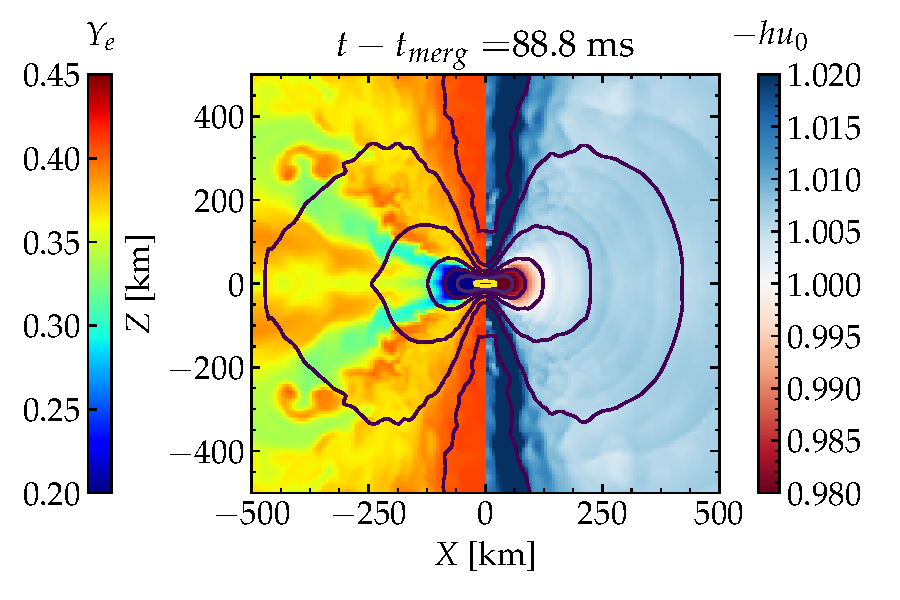
\includegraphics[width=0.49\textwidth]{slices/slice_xz_ye_hu_1.pdf}
    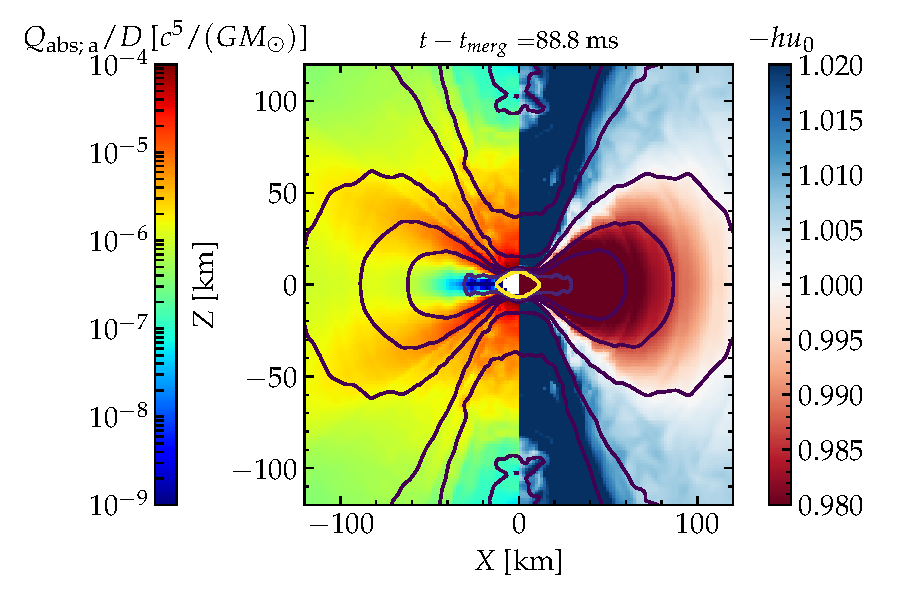
\includegraphics[width=0.49\textwidth]{slices/slice_xz_abs_energy_hu_3.pdf}
    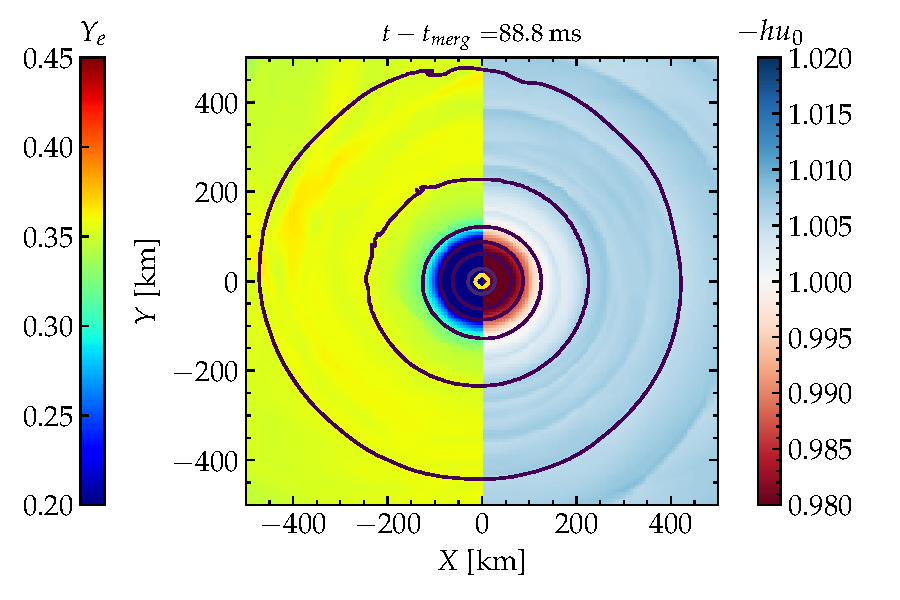
\includegraphics[width=0.49\textwidth]{slices/slice_xy_ye_hu_1.pdf}
    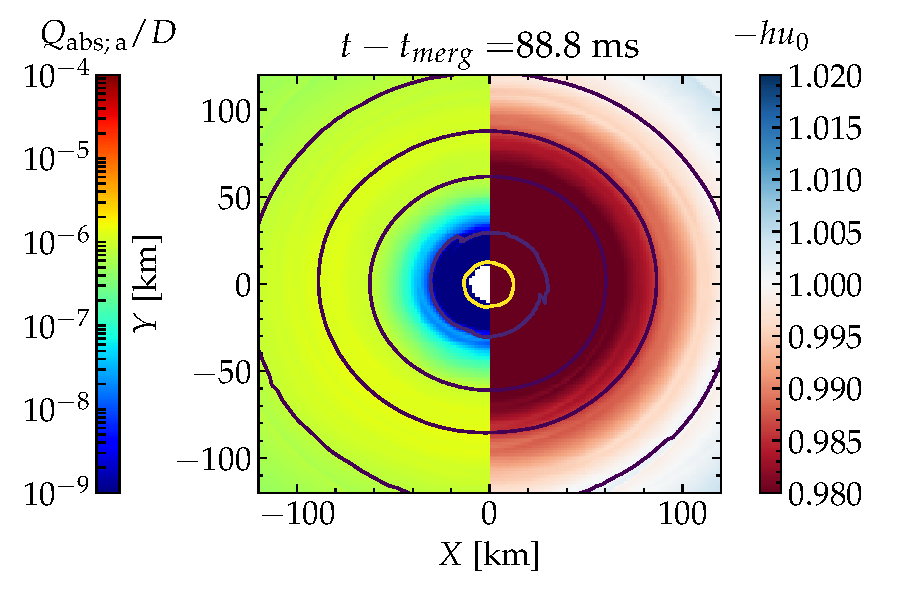
\includegraphics[width=0.49\textwidth]{slices/slice_xy_abs_energy_hu_3.pdf}
    \caption{Snapshot of the $(x,z)$ and $(x,y)$ slices of the BLh $q=1$ model at 
        ${\sim}89\,$ms after merger. Left panels: electron fraction and
        $-hu_0$. High $Y_e$ values indicate neutrino
        postprocessing and irradiation. The $-hu_0>1$ indicates the
        material that gains enough energy to become unbound at
        infinity. 
        %
        Right: $-hu_0$ and the absorption energy rate $Q_{\text{abs};\:\bar{\nu}_e}$ 
        of electron antineutrinos normalized to the fluid density $D$.
    }
    %
    \label{fig:slice:heating_hu}
\end{figure*}

In this section we investigate in detail the 
high electron fraction, polar component of the \acp{SWW}.
We propose that this outflow is mostly driven by the neutrino 
reabsorption, rather than by the dynamical mechanism responsible for the bulk of the 
\ac{SWW}.

The presence of the baryonic winds developing on the timescale of $\mathcal{O}(10)$~ms
and driven by the neutrino absorption above the remnant, where the neutrino flux is strong 
was reported before \citep[\eg][]{Perego:2014fma}. 

In this section we focus of the feducial model BLh $q=1.00$ (SR). 

In the left column of plots in Fig.~\ref{fig:slice:heating_hu} we compare 
the the Bernoulli parameter, 
$-hu_t$ (see Sec.\ref{sec:method:Bernoulli}), and the fluid electron 
fraction. 

In the right column of plots in Fig.~\ref{fig:slice:heating_hu} we compare 
the the Bernoulli parameter with the heating energy rate due to electron anti-neutrino absorption 
$Q_{\text{abs};\:\bar{\nu}_e}$ (see Sec.~\ref{method:M0:eq_for_Q}) divided by with 
$D=W\rho\sqrt{\gamma}$ (fluid's conserved rest-mass density)
We observe that the electron fraction in the polar region with angle 
from binary plane $\theta>60^{\circ}$ reaches $Y_e\sim0.35$ due to the absorption of 
electron-type neutrinos.
The strongest neutrino heating occurs in the vicinity of the remnant at densities 
$\rho\sim10^{11}$~\gcm, that roughly correspond to the region where neutrinos decouple,
the so-called neutrinosphere \citep{Endrizzi:2019trv}.

In Fig.~\ref{fig:slice:heating_hu} we compare the Bernoulli parameter, 
$-hu_t$ (see Sec.\ref{sec:method:Bernoulli}), that is always plotted 
on the right half of a panel, with the electron fraction (left 
column of plots and heating energy rate due to electron anti-neutrino absorption 
$Q_{\text{abs};\:\bar{\nu}_e}$ divided by with $D=W\rho\sqrt{\gamma}$ 
(fluid's conserved rest-mass density).
The observed correlation between the $E_\nu/D$ \red{???} and $-h u_t$ further suggests, 
that the outflow around the polar axis is driven by the neutrino absorption. 
Additionally, we found that if the neutrino absorption is not included into the 
simulation, \eg, using leakage only, the \nwind{} is absent. 
%% --- 
The collimated polar outflow can be further boosted and stabilized by the presence of the 
strong magnetic fields \citep{Bucciantini:2011kx,Ciolfi:2020hgg,Mosta:2020hlh}.
%% ---
Notably, there is not clear distinction between the \nwind{} and \ac{SWW}, especially 
at the intermediate latitudes ($\theta \sim 45^{\circ}$), where both mechanisms types of 
ejecta are present, and both, neutrino absorption and dyanmical effects driving the \ac{SWW} 
are contributing. 
%% --- 
In order to compute the mass flux of the \nwind{} an additional criterion is required. 
We consider two physically motivated criteria, the geometrical, flaggin the part of the \ac{SWW} 
and \nwind{} if it is polar, \ie, $\theta>60^{\circ}$, and the composition criterion, $Y_e > 0.35$.
%% --- 
We find that the \nwind{} is not a steady state outflow, contrary to the bulk of the \ac{SWW}.
After the initial strong rise, the mass flux rapidly decays in time, and for most models stops 
by the end of the simulations. This behaviour is independent of the criterion we use. 
We attribute it to the rise of the baryon loading above the remnant as the material gets lifted 
by thermal pressure from the disk.
The total mass of the \nwind{} is ${\sim}10^{-3}-10^{-4}M_{\odot}$. Its properties resemble those 
reported in e.g. \citet{Dessart:2008zd,Perego:2014fma,Fujibayashi:2020dvr}
Notably, in some of the works, the \nwind{} was found to require longer timescales to develop, 
achieving the quasi-steady state. 
This can be attributed to the strict criteria to isolate the \nwind{} and by the absence of the 
\ac{SWW} in other works. 
Additionally, our simulations might not be sufficiently long to achieve the donditions 
sufficient for the development of the quasi-steady state \nwind{}.
%% Additionally, as our models are at most $\sim100$~ms long, the conditions required for the steady 
%% state \nwind{} might not been achieved.


%% =======================================================
%%
%%                   Disc structure
%%
%% =======================================================


\section{Remnant disk structure}

\begin{figure}[t]
    \centering
    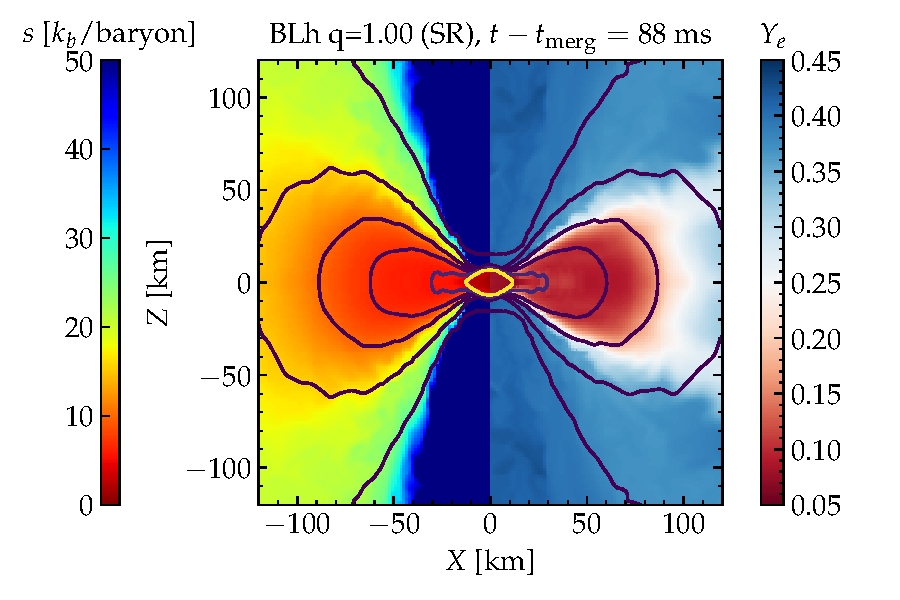
\includegraphics[width=0.49\textwidth]{disk/final_structure/slice_xz_entr_ye_blh_q1_rl3.pdf}
    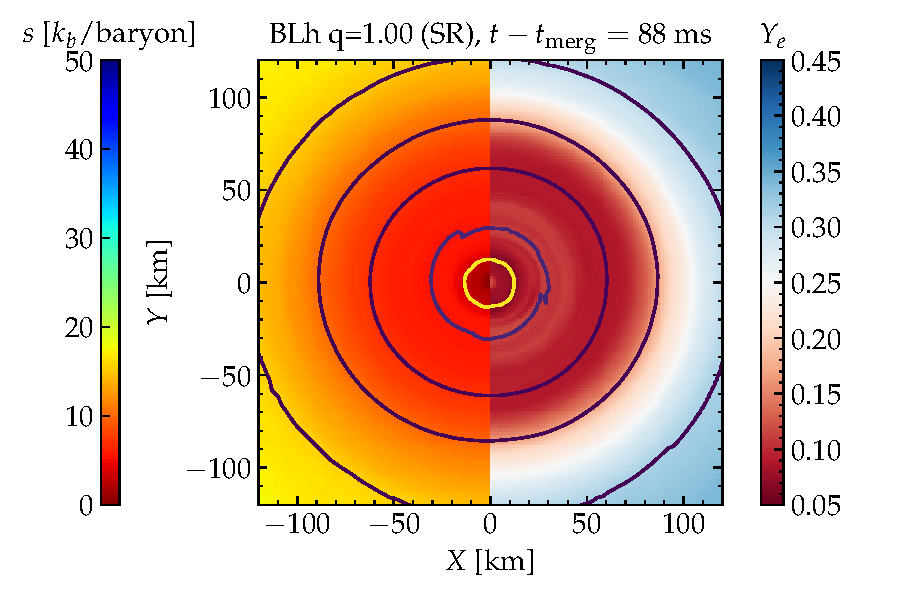
\includegraphics[width=0.49\textwidth]{disk/final_structure/slice_xy_entr_ye_blh_q1_rl3.pdf}
    \caption{Entropy and electron fraction on the $(x,z)$ (top) and
        $(x,y)$ planes (bottom) for the remnant of BL $q=1$ at the end
        of the simulation. Each plot is divided vertically, with entropy
        being color-coded on the left and electron fraction on the
        right. Solid contours stand for rest muss density. Counting from
        the center, the values are $[10^{13}, 10^{12}, 10^{11}, 10^{10},
        10^{9}]$ g cm$^{-3}$, with the inner most contour encompassing
        the remnant.
        (Adapted from \citet{Nedora:2020pak})
    }  
    \label{fig:snapshots_xy_ye_entr}
\end{figure}

\begin{figure*}[t]
    \centering 
    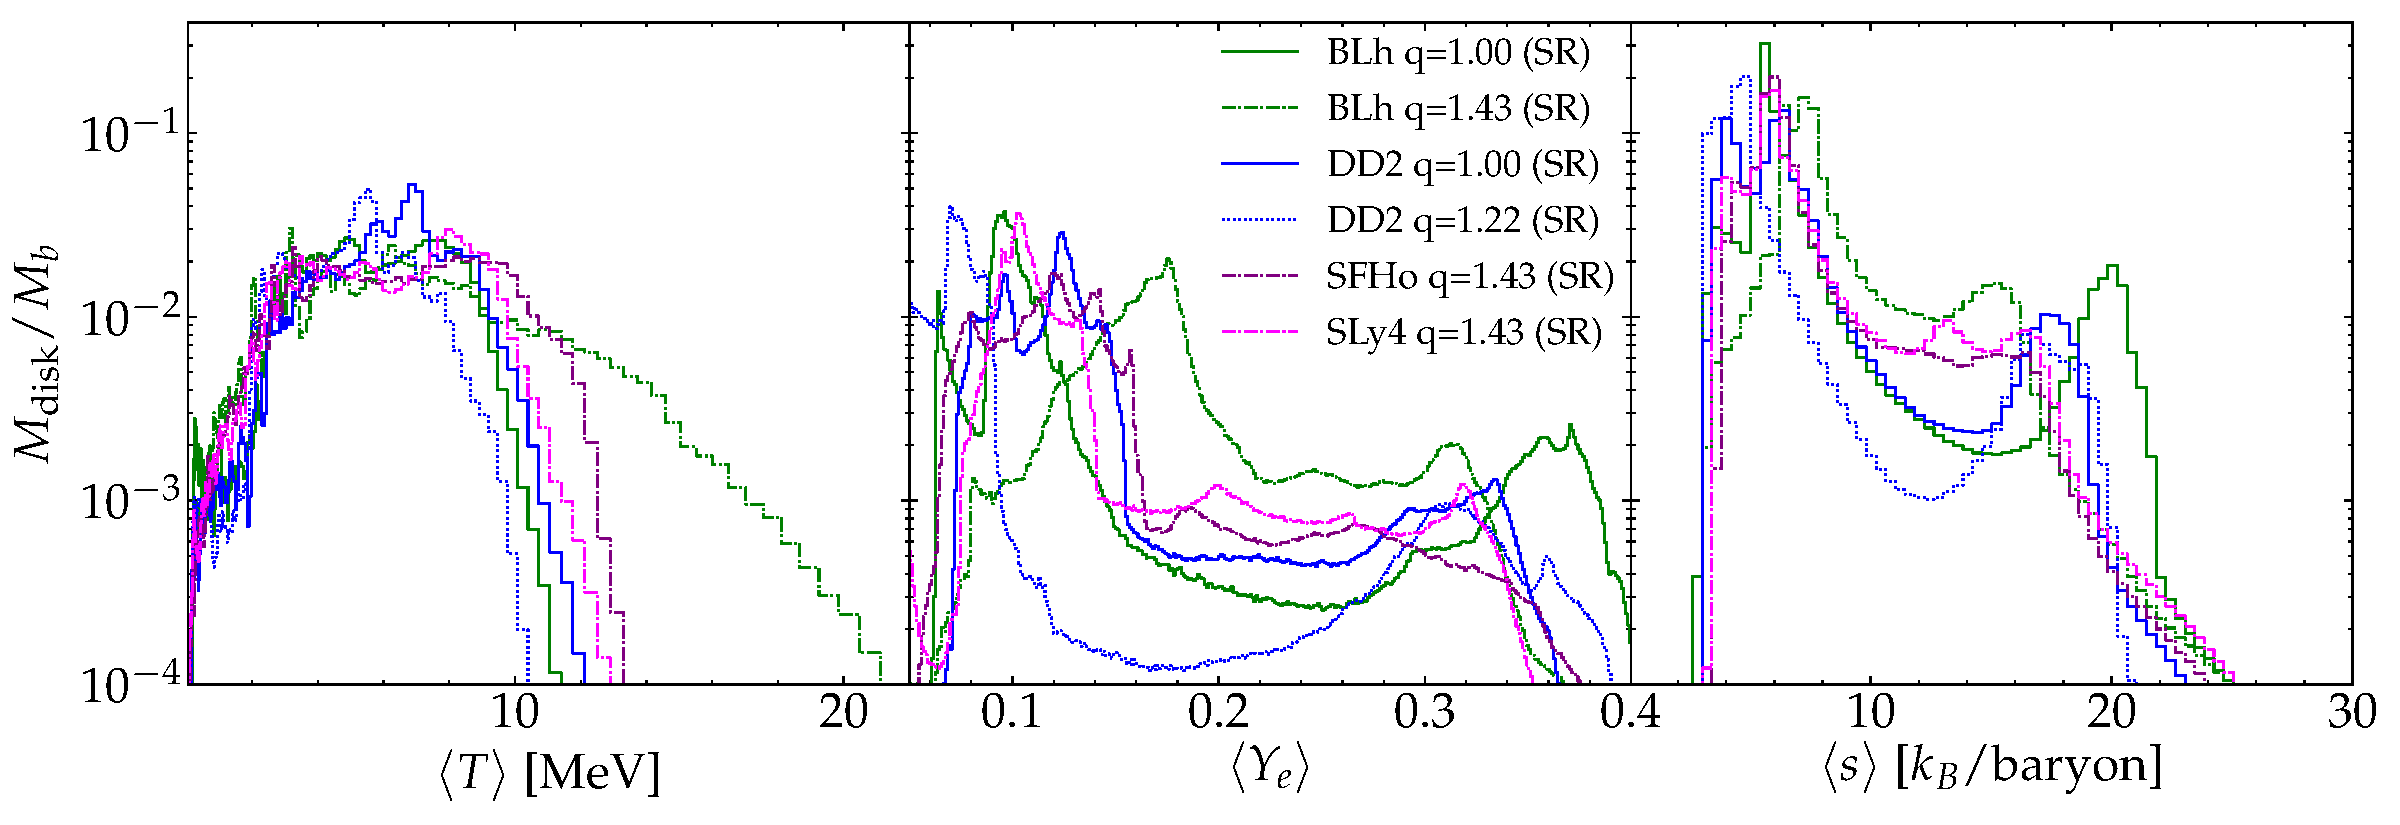
\includegraphics[width=0.95\textwidth]{disk/final_structure/disk_hist_shared.pdf}
    \caption{Composition of the disks at the end of the long-lived
        remnants simulations. The histograms refer to the temperature $T$
        (left),
        electron fraction $Y_e$
        (middle) and entropy $s$ (right).
        (Adapted from \citet{Nedora:2020pak})
    }
    \label{fig:final_disk_struct_hist_long}
\end{figure*}

In this section we discuss the final structure and properties of the disk, 
focusing on the models with long-lived \ac{MNS} remnants.
The properties are extracted at typical time $\sim60{-}100$~ms after merger.

We find that the generally the disk is optically thick.
The disk' RMS openning appears to be independent of the \ac{EOS} and \mr{} and
is $\langle\theta\rangle_{\text{rms}}\sim60^{\circ}$. 
The radial extend of the disk, however increases with the \ac{EOS} softness and 
binary \mr{}.
Similarly, the final disk mass is larger for the unequal mass binaries, 
ranging overall between ${\sim}0.1M_{\odot}$ and ${\sim}0.4M_{\odot}$
(see Tab.~\ref{tab:sim})..
Notably, for models with long-lived remnants the disk mass is larger,
that for the those with long-lived remnants. This can be attributed to the 
rapid accretion onto a \ac{BH} that removes $\sim50\%$ of the disk mass.
%% ---
We investigate the overall statistical properties of the disk mass for all our models
and those available in the literature in Sec.\ref{sec:results:Statistics:Mdisk}
\gray{
    The mean value of the disk mass in out models is 
    $\overline{M}_{\text{disk}}=(0.161 \pm 0.083)M_{\odot}$,
    where the standard deviation is also reported.
    %% ---
    Similarly to the dynamical ejecta we fit the disk masses with the 
    second order polynomial in $(q,\tilde{\Lambda})$.
    The coefficients of Eq.~\eqref{eq:fit:poly22}
    for this fit are given in Tab.~\ref{tab:fitpoly22coefs}.
    A more detailed study with various fitting formulas and extended
    datasets from the literature is reported in a companion paper.
}

Next, we consider the composition of the disk at the end of the simulation.
%% --- 
The mass-averaged temperature, electron fraction and entropy per baryon
are for several models are shown in Fig.~\ref{fig:final_disk_struct_hist_long}.
%% ---
We observe that the mass-weighted distribution of the entropy and electron 
fraction show a bimodal structure, which is more pronounced for the 
equal mass binaries. 
Regarding entropy, two peaks are present in the distribution:
a peak low entropy $s\sim5-10k_B/$baryon, that depends weakly of the 
\ac{EOS} and \mr{} and corresponds to the bulk, mildly shocked, material. 
The second peak is found at higher entropy, $s\sim15-22k_B/$baryon.
It corresponds fo the strongly shocked material and is more prominent 
in models with softer \ac{EOS}.
Notably, in the models with higher \mr{}, the second peak is located 
at lower $s$.
The mass-weighted distribution of the electron fraction 
displays a similar double-peak structure.
The low $Y_e$ peak that corresponds to the neutrino-shielded part of the 
disk is located around the $Y_e\sim0.1$.
The high $Y_e$ peak is located at $Y_e\sim0.3-0.4$ and corresponds to the outer parts of the disk, subjected to a strong neutrino irradiation.

In Fig.~\ref{fig:snapshots_xy_ye_entr} we show the electron fraction 
and entropy per baryon on the $xy$ and $xz$ slices of the equal 
mass model with BLh \ac{EOS}.
The plot shows, that the two peaks in the mass-weighted distribution 
of electron fraction and entropy correspond to different regions within the disk.

Overall, the most of the disk matter has temperature of $T\sim 1-10\,$MeV, with the innermost parts being hotter then the outer outermost. 
However, the disk temperature distribution appears to be largely independent of the \ac{EOS} and \mr{}

\red{Paragraph on the secular ejecta has been moved to 
    GW170817 application}





%% =======================================================
%%
%%                   Conclusion
%%
%% =======================================================




%% ========================================================================================

\section{Statistics of the \ac{DE} parameters and disk mass}

\red{CONTENT OF THE FIT PAPER}


\section{Application to \GW{}}


\begin{figure*}[t]
    \centering 
    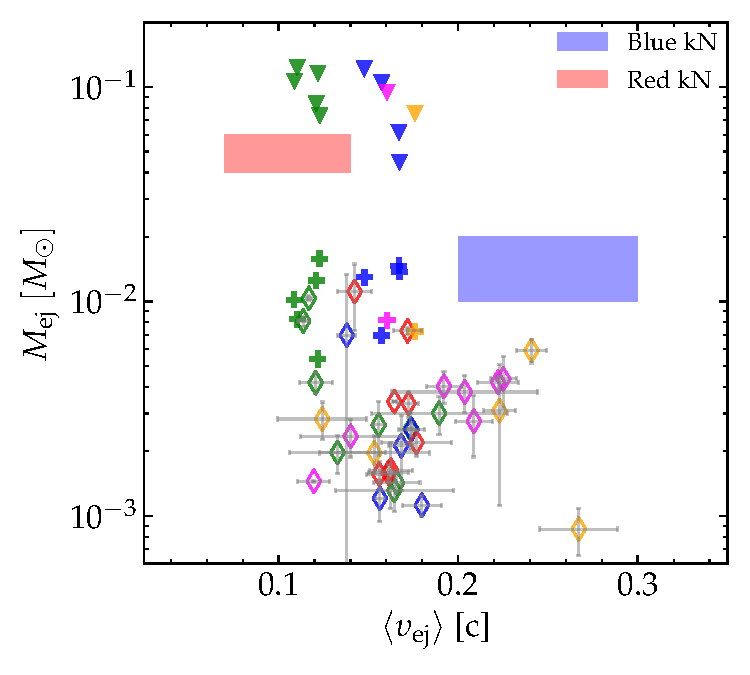
\includegraphics[width=0.48\textwidth]{ejecta_dyn/summary/ej_mej_vej_our2.pdf}
    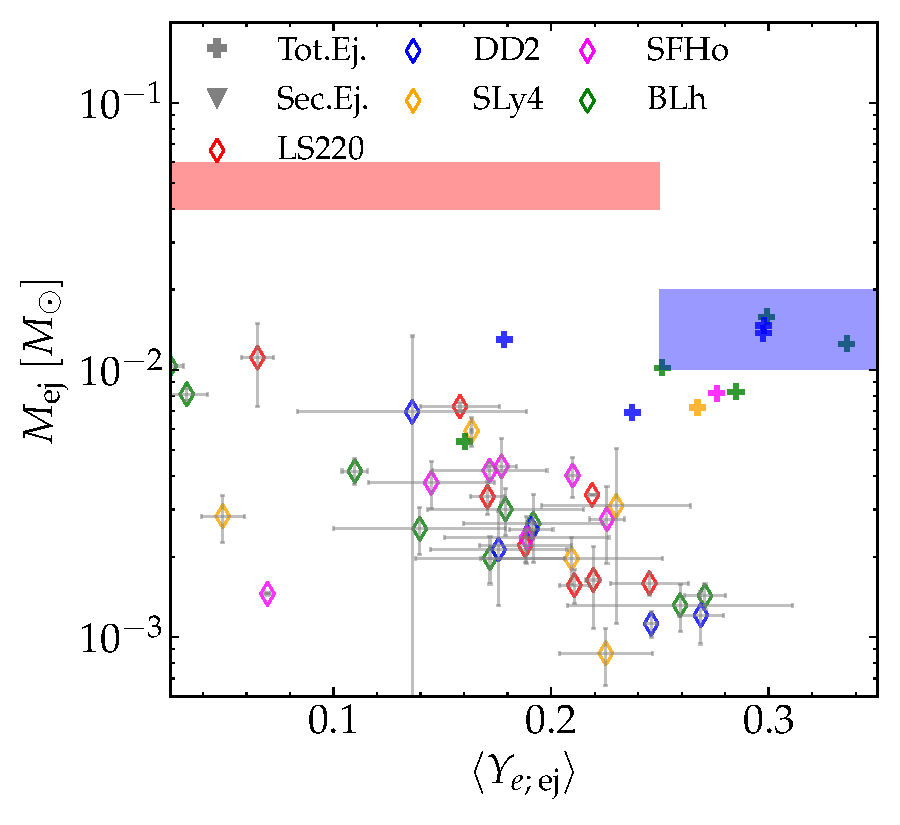
\includegraphics[width=0.48\textwidth]{ejecta_dyn/summary/ej_mej_yeej_our2.pdf}
    \caption{
        Summary of the ejecta properties of our models.
        %
        Diamonds mark the dynamical ejecta, crosses include the
        contribution of the \swind{} for the long-lived models, 
        triangles are an estimate of the total ejecta mass on a secular
        timescale, assuming $40\%$ of the disk mass is unbounded on
        secular timescales.         
        The ejecta mass is shown is terms of the mass-averaged velocity
        (left) and of the averaged electron fraction (right).
        %
        The filled blue and red patches are the expected values of
        ejecta mass and velocity for blue and red components of
        AT2017gfo compiled by \cite{Siegel:2019mlp}, based on
        \cite{Villar:2017wcc}. 
        Adopted from \citet{Nedora:2020pak}.
    }
    %
    \label{fig:ejecta:dyn:ds_sww}
\end{figure*}


%% from main paper, referencing the fitpaper Poly22 fits and SWW + DE
\red{THis can be augmented with Radio afterglow}

%% === FROM DYNAMICAL EJECTA SECTION of MAIN PAPER
Here we discuss the application of our results to \GW{}.


\subsection{Dynamical Ejecta}


%% ---
First, we asses the ejecta parameters that our fitting models, 
obtained in section \ref{sec:ejecta_disk_statisitcs} would provide for the \GW{}.
%% --- 
Considering the $90\%$ credible intervals estimated for $q$ and $\tilde{\Lambda}$ 
from LIGO-Virgo GW analysis
\citep{TheLIGOScientific:2017qsa,Abbott:2018wiz,De:2018uhw,Abbott:2018exr},
i.e.~$\tilde{\Lambda}=300_{-190}^{+500}$ and $q\in[1., 1.37]$. 
and using the errorbars formulas developed in \cite{Radice:2018pdn}, we find that
$\amd \in [0.72, 7.52] \times 10^{-3}\: M_{\odot}$
and
$\avd \in [0.16, 0.39]$c 
and 
$\ayd \in [0.11, 0.23]$.
Notably, these values do not agree with those inferred for \AT{} by the spherical, 
two-component kilonova models \citep{Villar:2017wcc}.
Analysis of a compiled set of kilonova fitting models provides a broad range of ejecta 
parameters \citep{Siegel:2019mlp}:
$M_{\text{ej}}^{\text{red}}\in(4, 6)\times10^{-2}M_{\odot}$ and
$\upsilon_{\text{ej}}^{\text{red}}\in(0.07, 0.14)$ for the red component, while
$M_{\text{ej}}^{\text{blue}}\in[1, 2]\times10^{-2}M_{\odot}$ and 
$\upsilon_{\text{ej}}^{\text{blue}}\in[0.2, 0.3]$ for the blue component.
%% ---
With respect to our results for \ac{DE}, however, 
none of the kilonova components can be well explained.
%% ---
In Fig.~\ref{fig:ejecta:dyn:ds_sww} we show the ejecta properties from
all our models (diamonds) and the parameters inferred from the
observations as red and blue boxes. 
%% --- 
With respect to the red component, we observe that \ac{DE} from our models 
have too high average velocities and not nearly enough mass.
This result suggests that an additional, low $Y_e$ ejecta component is required
in order to explain the \AT{} red component 
\citep{Perego:2017wtu,Kawaguchi:2018ptg,Nedora:2019jhl}.
%% --- 
A more thorough analysis of the \AT{} with better ejecta models and advanced
radiation transport kilonova simulations are not part of the present work 
and will be addressed in the future.


\subsection{\swind{}}


The \ac{SWW} could be a significant contributor to the \AT{}, assuming the remnant of 
\GW{} \ac{MNS} merger survived for $\mathcal{O}(100)$~ms.
%% ---- 
In Fig.~\ref{fig:ejecta:dyn:ds_sww} we report the total
(dynamical+\swind{}) ejecta mass and mass-averaged velocity for the
simulated long-lived BNS (crosses).
%% ---
Notably, the total ejecta mass of three of our models, 
BLh $q=1.18$, BLh $q=1.42$ and  DD2 is $q=1$ are in agreemnt with the epected values 
for the blue compoent of the \AT{} 
(obtained using the two-component fit \citep{Villar:2017wcc})

\red{
    [ LETTER STUFF COULD GO HERE ]
    a multi-component fitting model that explicitly accounts
    for the \swind{} can fit the early blue
    emission from AT2017gfo \citep{Nedora:2019jhl}
}

The high electron fraction of the \ac{SWW} however would result in a lanthanides-poor
composition of the outflow. Thus, the \ac{SWW} cannot explain the observed emission 
for the high opacity, lanthanides-rich material.
%% ---
Simulations with advanced physics of a \ac{MNS} mergers on a timescales $>100$~ms are 
required to asses the contribution from other outflow mechanisms, \red{that we will discuss below} 
\citep{Lee:2009uc,Fernandez:2015use,Siegel:2017nub,Fujibayashi:2017puw,Fernandez:2018kax,Radice:2018xqa}.


\subsection{Secular Ejecta}


On the timescale of seconds, much longer than the evolution of 
presented here simulations, the nuclear recombination can unbind 
a fraction of the disk mass. 
Analytical estimates and simulations with various approximations show that up tp ${\sim}40\%$ of the disk can be ejected via viscous processes with an typical velocity ${\lesssim}0.1\,$c
\citep{Lee:2009uc,Fernandez:2015use,Wu:2016pnw,Siegel:2017nub,Fujibayashi:2017puw,Fernandez:2018kax,Radice:2018xqa,Fujibayashi:2020dvr}.

Adapting the fix fraction of the $40\%$ of the disk mass, we estimate 
that about  ${\sim}0.05\, M_{\odot}$ would be ejected in a form of 
secular winds. We include this estimate for every simulation
with the long-lived \ac{MNS} remnant in Fig.~\ref{fig:ejecta:dyn:ds_sww} (lower triangles).
The estimated mass is sufficient to explain
the red component of AT2017gfo, as inferred from the two-components kN
models of \cite{Villar:2017wcc}. 







%% ---------------------
Sources with time delay are preferred by studies of very metal poor stars that indluded the time delay for r-process elements
to diffuse through ISM, \citep{Tarumi:2021xvw}. 
A winds from proto-nuetron are also contributors to the $r$-process budget \cite{Vincenzo:2021rvw}

\red{The remnant is losing anular momentum while disk gains on shortly after merger is due to gravitational torque \cite{Shibata:2019wef}}
